% ============================================================================
%  End-Term Project Report
%  Crop Disease Detection and Localized Treatment Recommendation
%  Using Deep Learning
%
%  HOW TO COMPILE
%  ---------------
%  This file has no local LaTeX distribution to test against in the
%  environment it was written in. It uses only mainstream, widely-available
%  packages (see preamble) and was written defensively for pdflatex. Easiest
%  path: upload this .tex file plus the figures/ folder to a new Overleaf
%  project and hit Recompile. Locally: pdflatex -> pdflatex (run twice for
%  the Table of Contents / List of Figures / cross-references to settle).
%
%  WHAT YOU MUST EDIT BEFORE SUBMITTING
%  -------------------------------------
%  1. The macros in the "EDIT THESE FIELDS" block below (title, names,
%     roll numbers, guide, specialization, month/year).
%  2. Section 6.10 "Output Screens" -- these are placeholder boxes. Run the
%     Streamlit app (`streamlit run App.py`) and drop in real screenshots.
%  3. Chapter 3 UML placeholders (Use-Case / Sequence) are simplified TikZ
%     diagrams meant as a faithful starting point -- adjust wording/flow to
%     match your final app if it has changed.
%  4. The reference list is representative of the tools/datasets/papers
%     actually used; add any further citations your guide asks for.
% ============================================================================

\documentclass[12pt,a4paper]{report}

% ---------- Fonts / encoding ----------
\usepackage[T1]{fontenc}
\usepackage[utf8]{inputenc}
\usepackage{times}

% ---------- Layout ----------
\usepackage[a4paper,margin=1in,bindingoffset=0.3in]{geometry}
\usepackage{setspace}
\onehalfspacing

% ---------- Graphics / diagrams ----------
\usepackage{graphicx}
\graphicspath{{figures/}{./figures/}}
\usepackage{tikz}
\usetikzlibrary{positioning,arrows.meta,shapes.geometric,calc,fit,shapes.symbols}
\usepackage{float}

% ---------- Tables ----------
\usepackage{booktabs}
\usepackage{longtable}
\usepackage{array}
\usepackage{multirow}
\usepackage{tabularx}

% ---------- Misc ----------
\usepackage{amsmath,amssymb}
\usepackage{xcolor}
\usepackage{enumitem}
\usepackage{listings}
\usepackage[labelfont=bf,font=small]{caption}
\usepackage{tocloft}
\usepackage{titlesec}
\usepackage{fancyhdr}
\usepackage{url}
\usepackage[hidelinks]{hyperref}

% ---------- Counters: Fig./Table numbered within chapter, e.g. Fig. 4.1 ----------
\counterwithin{figure}{chapter}
\counterwithin{table}{chapter}
\renewcommand{\figurename}{Fig.}

% ---------- Chapter heading style: "1. Introduction" not "Chapter 1" ----------
\titleformat{\chapter}[hang]{\normalfont\Huge\bfseries}{\thechapter.}{18pt}{\Huge}
\titlespacing*{\chapter}{0pt}{0pt}{28pt}

\setcounter{secnumdepth}{3}
\setcounter{tocdepth}{3}

% ---------- Header/footer ----------
\pagestyle{fancy}
\fancyhf{}
\fancyhead[R]{\small\thepage}
\fancyhead[L]{\small\nouppercase{\leftmark}}
\renewcommand{\headrulewidth}{0.4pt}

% ---------- Code listings ----------
\lstdefinestyle{pystyle}{
  language=Python,
  basicstyle=\ttfamily\scriptsize,
  keywordstyle=\color{blue!60!black}\bfseries,
  commentstyle=\color{gray!70!black}\itshape,
  stringstyle=\color{teal!70!black},
  showstringspaces=false,
  breaklines=true,
  breakatwhitespace=false,
  frame=single,
  rulecolor=\color{black!40},
  numbers=left,
  numberstyle=\tiny\color{black!50},
  numbersep=6pt,
  tabsize=4,
  captionpos=b,
  columns=fullflexible,
}
\lstset{style=pystyle}

% ---------- Placeholder figure for un-captured screenshots ----------
\newcommand{\ScreenshotPlaceholder}[2]{%
\begin{figure}[H]
\centering
\begin{tikzpicture}
\draw[dashed, thick, gray!70] (0,0) rectangle (13,#2);
\node[align=center, text width=11.5cm, gray!70, font=\itshape] at (6.5,{#2/2}) {Insert screenshot here:\\#1};
\end{tikzpicture}
\end{figure}%
}

% ============================================================================
%  EDIT THESE FIELDS
% ============================================================================
\newcommand{\ReportTitle}{Crop Disease Detection and Localized Treatment Recommendation Using Deep Learning}
\newcommand{\DegreeName}{BACHELOR OF TECHNOLOGY}
\newcommand{\BranchName}{COMPUTER SCIENCE \& ENGINEERING}
\newcommand{\SpecializationName}{[Specialization -- e.g. Artificial Intelligence \& Machine Learning]}
\newcommand{\SchoolName}{School of Computer Science}
\newcommand{\UniversityName}{University of Petroleum \& Energy Studies}
\newcommand{\UniversityAddress}{Bidholi, Via Prem Nagar, Dehradun, Uttarakhand}
\newcommand{\SubmissionMonth}{[Month]}
\newcommand{\SubmissionYear}{2026}
\newcommand{\GuideName}{[Guide's Name]}
\newcommand{\GuideDesignation}{[Guide's Designation]}
\newcommand{\StartMonthYear}{[Start Month, Year]}
\newcommand{\EndMonthYear}{[End Month, Year]}
\newcommand{\HodName}{[Name of HoD]}
\newcommand{\HodDept}{[Department Name]}
\newcommand{\DeanName}{[Dean, SoCS]}
\newcommand{\CourseCoordName}{[Course Coordinator Name]}
\newcommand{\ActivityCoordName}{[Activity Coordinator Name]}

% Team roster -- add/remove \StudentRow lines and table rows to match your
% actual group size (template default is up to four members).
\newcommand{\StudentAName}{Saksham Agrawal}
\newcommand{\StudentARoll}{[Roll No.]}
\newcommand{\StudentBName}{[Student 2 Name]}
\newcommand{\StudentBRoll}{[Roll No.]}
\newcommand{\StudentCName}{[Student 3 Name]}
\newcommand{\StudentCRoll}{[Roll No.]}
\newcommand{\StudentDName}{[Student 4 Name]}
\newcommand{\StudentDRoll}{[Roll No.]}

\begin{document}

% ============================================================================
%  FRONT MATTER
% ============================================================================
\pagenumbering{roman}

% ---------------------------- TITLE PAGE -----------------------------------
\begin{titlepage}
\centering
\vspace*{0.3cm}
{\Large \bfseries ``\ReportTitle''}\\[0.6cm]
{\large \itshape A}\\[0.2cm]
{\Large \itshape Project Report}\\[0.6cm]
{\itshape submitted in partial fulfillment of the}\\
{\itshape requirements for the award of the degree of}\\[0.8cm]
{\Large \bfseries \DegreeName}\\[0.2cm]
{\large \bfseries in}\\[0.2cm]
{\Large \bfseries \BranchName}\\[0.2cm]
{\large (\SpecializationName)}\\[1cm]
{\large \bfseries by}\\[0.8cm]

\begin{tabular}{|c|c|}
\hline
\textbf{Name} & \textbf{Roll No.} \\
\hline
\StudentAName & \StudentARoll \\
\hline
\StudentBName & \StudentBRoll \\
\hline
\StudentCName & \StudentCRoll \\
\hline
\StudentDName & \StudentDRoll \\
\hline
\end{tabular}\\[1cm]

{\itshape under the guidance of}\\[0.4cm]
{\large \bfseries \GuideName}\\
\GuideDesignation\\[1.2cm]

{\bfseries \SchoolName}\\
{\bfseries \UniversityName}\\
{\bfseries \UniversityAddress}\\[0.8cm]
{\bfseries \SubmissionMonth\ -- \SubmissionYear}
\vfill
\end{titlepage}

% ------------------------ CANDIDATE'S DECLARATION ---------------------------
\chapter*{CANDIDATE'S DECLARATION}
\addcontentsline{toc}{chapter}{CANDIDATE'S DECLARATION}

I/We hereby certify that the project work entitled \textbf{``\ReportTitle''} in partial
fulfilment of the requirements for the award of the Degree of \DegreeName\ in
\BranchName\ with specialization in \SpecializationName\ and submitted to the
Department of Systemics, \SchoolName, \UniversityName, Dehradun, is an
authentic record of my/our work carried out during a period from
\textbf{\StartMonthYear} to \textbf{\EndMonthYear} under the supervision of
\textbf{\GuideName, \GuideDesignation}.

The matter presented in this project has not been submitted by me/us for the
award of any other degree of this or any other University.

\vspace{0.6cm}
\noindent
\begin{tabular}{@{}p{7cm}@{}}
\StudentAName\ (\StudentARoll) \\[2pt]
\StudentBName\ (\StudentBRoll) \\[2pt]
\StudentCName\ (\StudentCRoll) \\[2pt]
\StudentDName\ (\StudentDRoll)
\end{tabular}

\vspace{1cm}
\noindent This is to certify that the above statement made by the candidate(s) is
correct to the best of my knowledge.

\vspace{1.2cm}
\noindent
\begin{minipage}{0.45\textwidth}
Date: \underline{\hspace{3.5cm}}
\end{minipage}
\begin{minipage}{0.45\textwidth}
\raggedleft
\textbf{(\GuideName)}\\
Project Guide
\end{minipage}

% ----------------------------- ACKNOWLEDGEMENT ------------------------------
\chapter*{ACKNOWLEDGEMENT}
\addcontentsline{toc}{chapter}{ACKNOWLEDGEMENT}

We wish to express our deep gratitude to our guide \textbf{\GuideName}, for all the
advice, encouragement, and constant support given throughout this project. This
work would not have been possible without the guidance and valuable
suggestions received at every stage -- from framing the problem, to choosing an
honest evaluation methodology, to reviewing the final system.

We sincerely thank our respected \textbf{\HodName}, Head of Department,
\textbf{\HodDept}, for the support extended in carrying out this project.

We are also grateful to \textbf{\DeanName}, Dean, \SchoolName, \UniversityName,
for providing the necessary facilities to carry out this project successfully.
We also thank our Course Coordinator, \textbf{\CourseCoordName}, and our
Activity Coordinator, \textbf{\ActivityCoordName}, for their timely support and
information during the completion of this project.

Finally, we would like to thank our friends and family for their patience,
encouragement, and constructive feedback throughout the duration of this work.

\vspace{0.8cm}
\begin{center}
\begin{tabular}{|c|c|c|c|c|}
\hline
\textbf{Name} & \StudentAName & \StudentBName & \StudentCName & \StudentDName \\
\hline
\textbf{Roll No.} & \StudentARoll & \StudentBRoll & \StudentCRoll & \StudentDRoll \\
\hline
\end{tabular}
\end{center}

% --------------------------------- ABSTRACT ---------------------------------
\chapter*{ABSTRACT}
\addcontentsline{toc}{chapter}{ABSTRACT}

Timely and accurate diagnosis of crop diseases is one of the highest-leverage
interventions available to smallholder farmers, yet expert diagnostic
knowledge rarely reaches the field in time to prevent yield loss. This project
presents an end-to-end, bilingual (Hindi/English) web application that lets a
farmer photograph a diseased leaf and receive, within seconds, a disease
diagnosis with a confidence score, a facts-based severity assessment, a
localized and weather-aware treatment plan, and a spoken audio summary of both.

The classification core of the system was developed and rigorously evaluated
on the \textbf{PlantVillage} dataset (Kaggle: \texttt{emmarex/plantdisease}),
restricted here to \textbf{15 disease/healthy classes} spanning Pepper (bell),
Potato, and Tomato, comprising 20{,}638 leaf images (20{,}624 after exact-duplicate
removal). Two convolutional architectures were built, trained, and compared
under an identical, stratified 70/15/15 train/validation/test protocol: a
VGG-style \textbf{custom CNN} trained from scratch, and an \textbf{EfficientNetB3}
transfer-learning model fine-tuned in two stages. On a held-out test set of
3{,}094 unseen images, the custom CNN achieved \textbf{95.51\% accuracy}
(94.86\% balanced accuracy, 94.59\% macro-F1, 99.81\% top-3 accuracy) and was
selected as the deployment model; EfficientNetB3 reached 87.10\% accuracy but
offered roughly \textbf{4.3$\times$ lower CPU inference latency}. Both models
were exported to \texttt{.keras}, \texttt{.h5}, and quantized \texttt{TFLite}
(fp32/fp16) formats, with the exported models re-verified against the
original Keras models for prediction fidelity before being reported as usable.

Around this model, the application layer adds a facts-based severity engine
(driven by pathogen type, curability, spread rate, and yield impact rather
than model confidence), a location- and weather-aware treatment planner backed
by a large language model, browser-geolocation and manual-address handling via
OpenStreetMap Nominatim, live weather context via Open-Meteo, and text-to-speech
narration via gTTS -- all switchable between Hindi and English.

The report documents the full pipeline: dataset preparation and exploratory
analysis, model architecture and training methodology, quantitative evaluation
(including confusion analysis, calibration, and Grad-CAM explainability), the
system's software architecture, and its implementation. It also states plainly
the model's principal limitation, which the evaluation itself surfaces: PlantVillage
is a lab-collected, uniform-background benchmark, and published literature
shows that models trained on it can lose substantial accuracy on
field-collected photographs. Recommendations for closing this gap -- field-image
validation, confidence-based abstention, and periodic retraining -- are given
in Chapter~7.

% ------------------------------ TOC / LOF / LOT -----------------------------
\tableofcontents
\clearpage
\listoffigures
\clearpage
\listoftables
\clearpage

\pagenumbering{arabic}

% ============================================================================
\chapter{Introduction}
% ============================================================================

\section{Background}
Plant diseases destroy an estimated 10--40\% of global crop yield every year,
and the gap between when a disease first appears on a leaf and when a farmer
can access expert diagnosis is often the difference between a controllable
outbreak and a lost harvest. Smartphone cameras and cheap mobile data have
made a different intervention possible: image-based diagnosis, running as a
model on a server or on-device, that gives a preliminary diagnosis in seconds
instead of days. Early work by Mohanty et al.~\cite{mohanty2016} demonstrated
that convolutional neural networks trained on the PlantVillage dataset could
classify 26 diseases across 14 crop species with over 99\% accuracy on
held-out PlantVillage images -- a result that this project's own evaluation
(Chapter~6) reproduces at a similar order of magnitude, and whose important
caveat (lab images are not field images) this project also inherits and
discusses honestly.

\section{Problem Statement}
A diagnosis alone is of limited use to a farmer without two further pieces of
information: \emph{how urgently must I act}, and \emph{what, specifically, do
I do about it, here, now}. Most academic disease-classification work stops at
the first question. This project treats the classification model as one
component of a larger decision-support pipeline that also answers the second
question -- severity and a concrete, localized, weather-aware treatment plan --
and delivers both in a language and format (including audio) usable by a
non-technical, potentially low-literacy user in the field.

\section{Objectives}
\subsection{Main Objective}
To design, train, evaluate, and deploy a deep-learning-based crop disease
diagnosis system that couples an image classifier with severity scoring and a
localized, weather-aware treatment recommendation engine, delivered through a
bilingual (Hindi/English) web interface with audio output.

\subsection{Sub-Objectives}
\begin{itemize}[leftmargin=*]
    \item Curate and analyze a labeled leaf-image dataset (PlantVillage) and
    quantify class imbalance, image quality, and potential dataset shortcuts.
    \item Design, train, and rigorously compare two CNN architectures --
    a hand-built CNN and a transfer-learning model -- under an identical,
    leakage-free evaluation protocol.
    \item Evaluate the models beyond raw accuracy: balanced accuracy, macro-F1,
    calibration, confusion structure, and explainability (Grad-CAM).
    \item Export the chosen model to a deployment-ready, quantized format and
    verify that quantization does not silently degrade accuracy.
    \item Build a severity-scoring engine grounded in plant-pathology facts
    rather than model confidence.
    \item Build a treatment-recommendation engine that incorporates the
    farmer's location and current/forecast weather.
    \item Provide the entire experience -- text and audio -- in Hindi and English.
\end{itemize}

\section{Scope of the Project}
The classification scope of this report is the 15-class Pepper/Potato/Tomato
subset of PlantVillage that the training notebook (Section~4.1) targets; this
is the dataset and set of classes referred to throughout Chapters~4 and~6.
The application scope covers the full farmer-facing workflow: image upload,
diagnosis, severity, location capture, weather context, treatment-plan
generation, and audio playback. Field-image generalization, multi-leaf/multi-disease
detection, and native mobile apps are treated as future work (Chapter~7), not
as part of the delivered system.

\section{Organization of the Report}
Chapter~2 reviews existing approaches and motivates the proposed system.
Chapter~3 presents the system's architecture and design artifacts. Chapter~4
covers dataset preparation, exploratory analysis, and model development in
detail -- this is the technical core of the project, drawn directly from the
training notebook. Chapter~5 describes the software implementation of the web
application. Chapter~6 presents quantitative results and output screens.
Chapter~7 discusses limitations and future work, and Chapter~8 concludes.

% ============================================================================
\chapter{System Analysis}
% ============================================================================

\section{Existing Systems}
Most publicly documented plant-disease-recognition systems fall into one of
two categories. The first is research prototypes that report a single
top-line accuracy number on PlantVillage or a similar lab-collected dataset
and stop there, without discussing calibration, confusion structure, or the
well-documented gap between lab and field performance
(Ferentinos~\cite{ferentinos2018}; Mohanty et al.~\cite{mohanty2016}). The
second is commercial or NGO-built mobile apps that provide a diagnosis but
little else -- no severity context, no localized treatment advice, and
frequently no offline or low-resource-language support, which limits their
usefulness to exactly the population (smallholder, non-English-speaking
farmers) that stands to benefit most.

\section{Motivation for the Proposed System}
A model that outputs ``\texttt{Tomato\_\_\_Late\_blight}, 92\% confidence'' is
not directly actionable. The motivating idea behind this project is that a
useful farmer-facing system needs three additional layers on top of
classification: (1) a severity signal so the farmer knows how urgently to
act, (2) a treatment recommendation specific to their crop, disease, region,
and current weather, and (3) a delivery format -- language and audio -- that
does not assume literacy in English or even in written Hindi.

\section{Proposed System}
The proposed system is a Streamlit-based web application that:
\begin{enumerate}[leftmargin=*]
    \item accepts an uploaded leaf photograph and classifies it using a
    CNN trained and evaluated as described in Chapter~4;
    \item computes a deterministic, facts-based severity level for the
    predicted condition;
    \item captures the farmer's location (GPS or manual entry) and current
    weather conditions;
    \item generates a localized treatment plan via a large language model,
    conditioned on crop, condition, severity, location, and weather;
    \item renders both the diagnosis summary and the treatment plan as
    speech, in the user's chosen language; and
    \item presents the entire experience in a bilingual (Hindi/English)
    interface that can be toggled at any point.
\end{enumerate}

\section{Modules Overview}

\subsection{Disease Classification Module}
Takes a preprocessed leaf image and returns a predicted class and confidence
score using the trained CNN (Chapter~4). This is the only module whose output
directly depends on the trained model weights; every other module consumes
its output.

\subsection{Severity Assessment Module}
Maps the predicted condition to a severity level using a lookup table of
plant-pathology facts (pathogen type, curability, spread rate, and yield
impact) rather than the model's confidence score, so that the same diagnosed
disease always receives the same severity regardless of how confident any
particular prediction happened to be.

\subsection{Localized Treatment Recommendation Module}
Given the crop, condition, severity, location, and weather context, calls a
hosted large-language-model API to generate a treatment plan appropriate to
the farmer's region and current conditions (locally available products,
timing of intervention, etc.), in the selected language.

\subsection{Location and Weather Module}
Resolves the farmer's location either from browser geolocation (reverse
geocoded) or a manually typed place name (forward geocoded), and fetches a
yesterday/today/tomorrow weather summary for that location to condition the
treatment plan on real, current conditions rather than generic seasonal advice.

\subsection{Multilingual Interface Module}
Drives every user-facing string in the application from a single translation
table, toggled at runtime between Hindi and English, with stale
results (previous predictions, plans, and audio) invalidated automatically on
a language switch.

\subsection{Text-to-Speech Module}
Converts the diagnosis summary and the treatment plan into spoken audio, so
that the output of the system is usable by farmers who may not be comfortable
reading dense text on a small screen.

% ============================================================================
\chapter{System Design}
% ============================================================================

\section{Technology Stack}
\begin{table}[H]
\centering
\caption{Technology stack of the deployed application.}
\begin{tabular}{@{}ll@{}}
\toprule
\textbf{Layer} & \textbf{Technology} \\
\midrule
UI / Web framework & Streamlit (Python) \\
Model training \& evaluation & TensorFlow / Keras (see Chapter~4) \\
On-device / lightweight inference & TensorFlow Lite (quantized, fp16) \\
Treatment-plan generation & Groq LLM API (\texttt{llama-3.3-70b-versatile}) \\
Geocoding (forward \& reverse) & OpenStreetMap Nominatim API \\
Weather data & Open-Meteo API \\
Text-to-speech & gTTS (Google Text-to-Speech) \\
Browser geolocation & \texttt{streamlit-js-eval} \\
Configuration / secrets & \texttt{python-dotenv} (\texttt{.env}) \\
\bottomrule
\end{tabular}
\end{table}

\section{System Architecture}
Figure~\ref{fig:architecture} shows the high-level architecture. The Streamlit
application is the single point of contact with the user; it fans out to five
independent engines, each of which is either a local computation (classification,
severity) or a thin client to an external API (treatment, location/weather,
speech). No engine depends on another directly -- they are all orchestrated by
the Streamlit app's session state, which keeps the design easy to reason about
and easy to extend with additional engines later.

\begin{figure}[H]
\centering
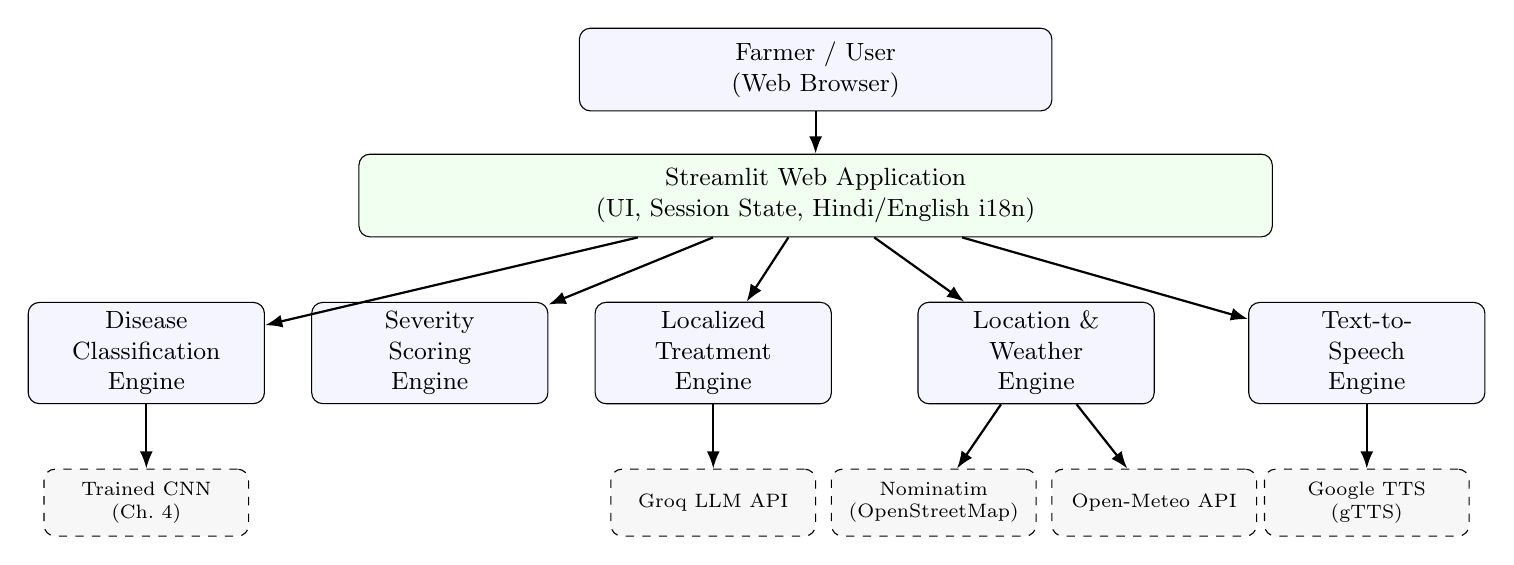
\begin{tikzpicture}[
  box/.style={draw, rounded corners, minimum width=3.0cm, minimum height=1.05cm, align=center, font=\small, fill=blue!4},
  ext/.style={draw, dashed, rounded corners, minimum width=2.6cm, minimum height=0.85cm, align=center, font=\scriptsize, fill=gray!6},
  arrow/.style={-{Latex[length=2.2mm]}, thick}
]
\node[box, minimum width=6cm] (user) at (0,7.4) {Farmer / User\\(Web Browser)};
\node[box, minimum width=11.6cm, fill=green!6] (app) at (0,5.8) {Streamlit Web Application\\(UI, Session State, Hindi/English i18n)};

\node[box] (cls) at (-8.5,3.8) {Disease\\Classification\\Engine};
\node[box] (sev) at (-4.9,3.8) {Severity\\Scoring\\Engine};
\node[box] (trt) at (-1.3,3.8) {Localized\\Treatment\\Engine};
\node[box] (wth) at (2.8,3.8) {Location \&\\Weather\\Engine};
\node[box] (spc) at (7.0,3.8) {Text-to-\\Speech\\Engine};

\node[ext] (trained) at (-8.5,1.9) {Trained CNN\\(Ch.~4)};
\node[ext] (groq) at (-1.3,1.9) {Groq LLM API};
\node[ext] (osm) at (1.5,1.9) {Nominatim\\(OpenStreetMap)};
\node[ext] (om) at (4.3,1.9) {Open-Meteo API};
\node[ext] (tts) at (7.0,1.9) {Google TTS\\(gTTS)};

\draw[arrow] (user) -- (app);
\draw[arrow] (app) -- (cls);
\draw[arrow] (app) -- (sev);
\draw[arrow] (app) -- (trt);
\draw[arrow] (app) -- (wth);
\draw[arrow] (app) -- (spc);
\draw[arrow] (cls) -- (trained);
\draw[arrow] (trt) -- (groq);
\draw[arrow] (wth) -- (osm);
\draw[arrow] (wth) -- (om);
\draw[arrow] (spc) -- (tts);
\end{tikzpicture}
\caption{High-level system architecture of the crop disease diagnosis and advisory platform.}
\label{fig:architecture}
\end{figure}

\section{Data Flow Diagram}

\subsection{Level 0 (Context Diagram)}
\begin{figure}[H]
\centering
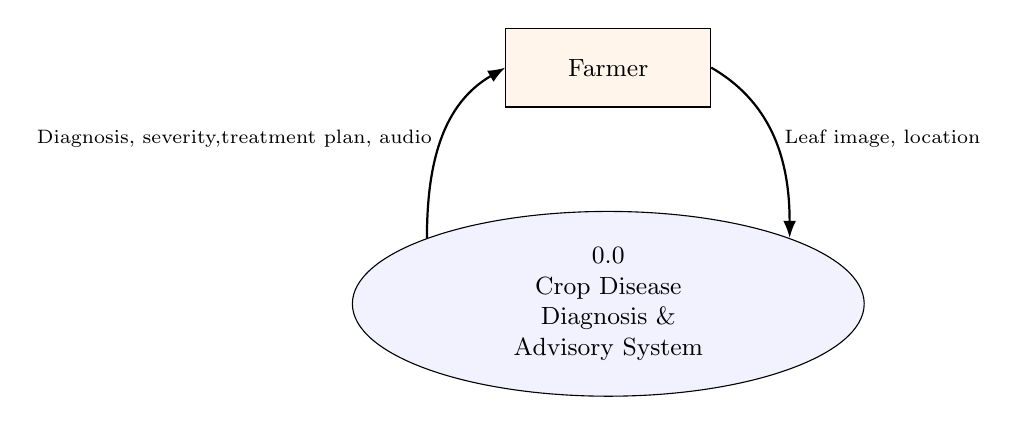
\begin{tikzpicture}[
  ent/.style={draw, minimum width=2.6cm, minimum height=1cm, align=center, font=\small, fill=orange!8},
  proc/.style={draw, ellipse, minimum width=6.5cm, minimum height=2cm, align=center, font=\small, fill=blue!5},
  arrow/.style={-{Latex[length=2.2mm]}, thick}
]
\node[ent] (farmer) at (0,3) {Farmer};
\node[proc] (system) at (0,0) {0.0\\Crop Disease\\Diagnosis \&\\Advisory System};
\draw[arrow] (farmer.east) to[out=-30,in=90] node[midway,right,font=\scriptsize]{Leaf image, location} (system.north east);
\draw[arrow] (system.north west) to[out=90,in=-150] node[midway,left,font=\scriptsize]{Diagnosis, severity,\\treatment plan, audio} (farmer.west);
\end{tikzpicture}
\caption{Level-0 (context) data flow diagram.}
\label{fig:dfd0}
\end{figure}

\subsection{Level 1}
\begin{figure}[H]
\centering
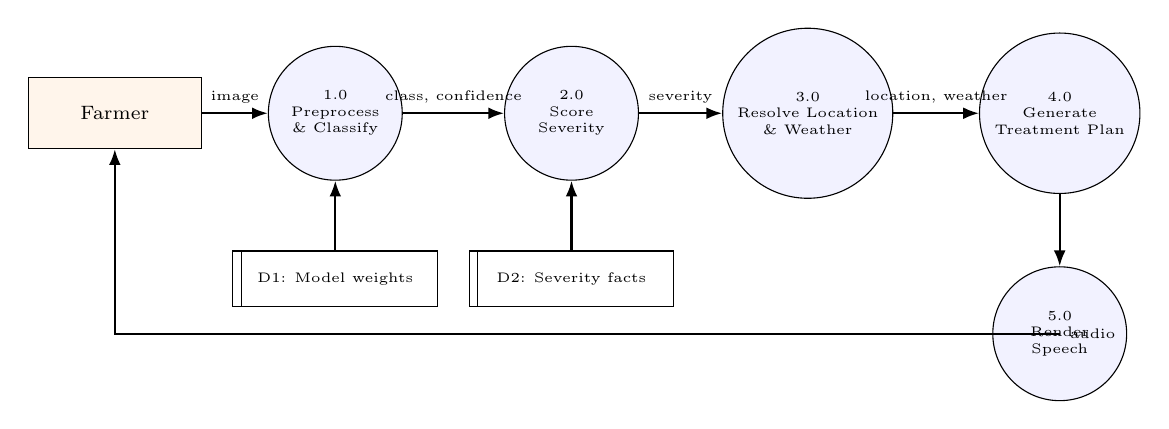
\begin{tikzpicture}[
  ent/.style={draw, minimum width=2.2cm, minimum height=0.9cm, align=center, font=\scriptsize, fill=orange!8},
  proc/.style={draw, circle, minimum size=1.7cm, align=center, font=\tiny, fill=blue!5},
  store/.style={draw, minimum width=2.6cm, minimum height=0.7cm, align=center, font=\tiny, path picture={
     \draw[black] ([xshift=3pt]path picture bounding box.north west) -- ([xshift=3pt]path picture bounding box.south west);}},
  arrow/.style={-{Latex[length=2mm]}, thick, font=\tiny}
]
\node[ent] (farmer) at (-6.4,3.2) {Farmer};
\node[proc] (p1) at (-3.6,3.2) {1.0\\Preprocess\\\& Classify};
\node[proc] (p2) at (-0.6,3.2) {2.0\\Score\\Severity};
\node[proc] (p3) at (2.4,3.2) {3.0\\Resolve Location\\\& Weather};
\node[proc] (p4) at (5.6,3.2) {4.0\\Generate\\Treatment Plan};
\node[proc] (p5) at (5.6,0.4) {5.0\\Render\\Speech};
\node[store] (d1) at (-3.6,1.1) {D1: Model weights};
\node[store] (d2) at (-0.6,1.1) {D2: Severity facts};

\draw[arrow] (farmer) -- node[above]{image} (p1);
\draw[arrow] (p1) -- node[above]{class, confidence} (p2);
\draw[arrow] (p2) -- node[above]{severity} (p3);
\draw[arrow] (p3) -- node[above]{location, weather} (p4);
\draw[arrow] (p4) -- (p5);
\draw[arrow] (p5) |- node[near start, right]{audio} (farmer |- p5) -- (farmer);
\draw[arrow] (d1) -- (p1);
\draw[arrow] (d2) -- (p2);
\end{tikzpicture}
\caption{Level-1 data flow diagram, decomposing the diagnosis-and-advisory process.}
\label{fig:dfd1}
\end{figure}

\section{Use Case Diagram}
\begin{figure}[H]
\centering
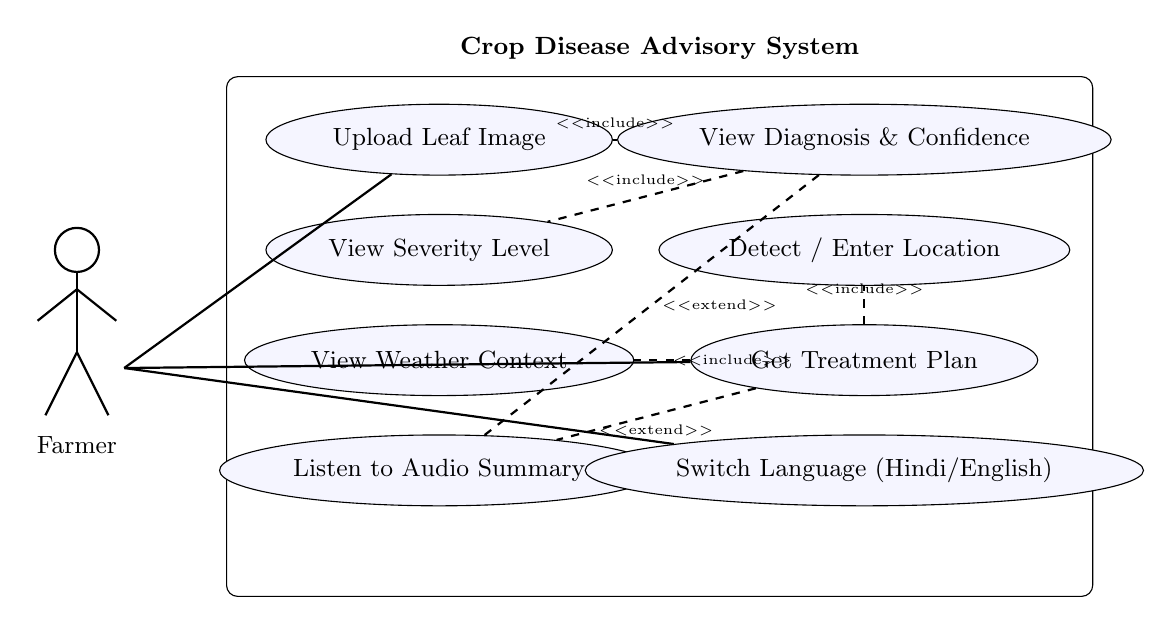
\begin{tikzpicture}[
  usecase/.style={draw, ellipse, minimum width=4.4cm, minimum height=0.9cm, align=center, font=\small, fill=blue!4},
  arrow/.style={thick}
]
% simple actor stick figure
\begin{scope}[shift={(-7.2,1.5)}]
  \draw[thick] (0,1.1) circle (0.28);
  \draw[thick] (0,0.82) -- (0,-0.2);
  \draw[thick] (0,0.6) -- (-0.5,0.2);
  \draw[thick] (0,0.6) -- (0.5,0.2);
  \draw[thick] (0,-0.2) -- (-0.4,-1.0);
  \draw[thick] (0,-0.2) -- (0.4,-1.0);
  \node[below, font=\small] at (0,-1.15) {Farmer};
\end{scope}

\node[draw, rounded corners, minimum width=11cm, minimum height=6.6cm] (boundary) at (0.2,1.5) {};
\node[above, font=\bfseries\small] at (0.2, 4.9) {Crop Disease Advisory System};

\node[usecase] (u1) at (-2.6,4) {Upload Leaf Image};
\node[usecase] (u2) at (2.8,4) {View Diagnosis \& Confidence};
\node[usecase] (u3) at (-2.6,2.6) {View Severity Level};
\node[usecase] (u4) at (2.8,2.6) {Detect / Enter Location};
\node[usecase] (u5) at (-2.6,1.2) {View Weather Context};
\node[usecase] (u6) at (2.8,1.2) {Get Treatment Plan};
\node[usecase] (u7) at (-2.6,-0.2) {Listen to Audio Summary};
\node[usecase] (u8) at (2.8,-0.2) {Switch Language (Hindi/English)};

\draw[arrow] (-6.6,1.1) -- (u1);
\draw[arrow] (-6.6,1.1) -- (u6);
\draw[arrow] (-6.6,1.1) -- (u8);
\draw[arrow,dashed] (u1) -- node[above,font=\tiny]{\textless\textless include\textgreater\textgreater} (u2);
\draw[arrow,dashed] (u2) -- node[above,font=\tiny]{\textless\textless include\textgreater\textgreater} (u3);
\draw[arrow,dashed] (u6) -- node[above,font=\tiny]{\textless\textless include\textgreater\textgreater} (u4);
\draw[arrow,dashed] (u6) -- node[right,font=\tiny]{\textless\textless include\textgreater\textgreater} (u5);
\draw[arrow,dashed] (u2) -- node[right,font=\tiny]{\textless\textless extend\textgreater\textgreater} (u7);
\draw[arrow,dashed] (u6) -- node[below,font=\tiny]{\textless\textless extend\textgreater\textgreater} (u7);
\end{tikzpicture}
\caption{Use-case diagram for the farmer-facing application.}
\label{fig:usecase}
\end{figure}

\section{Sequence Diagram}
\begin{figure}[H]
\centering
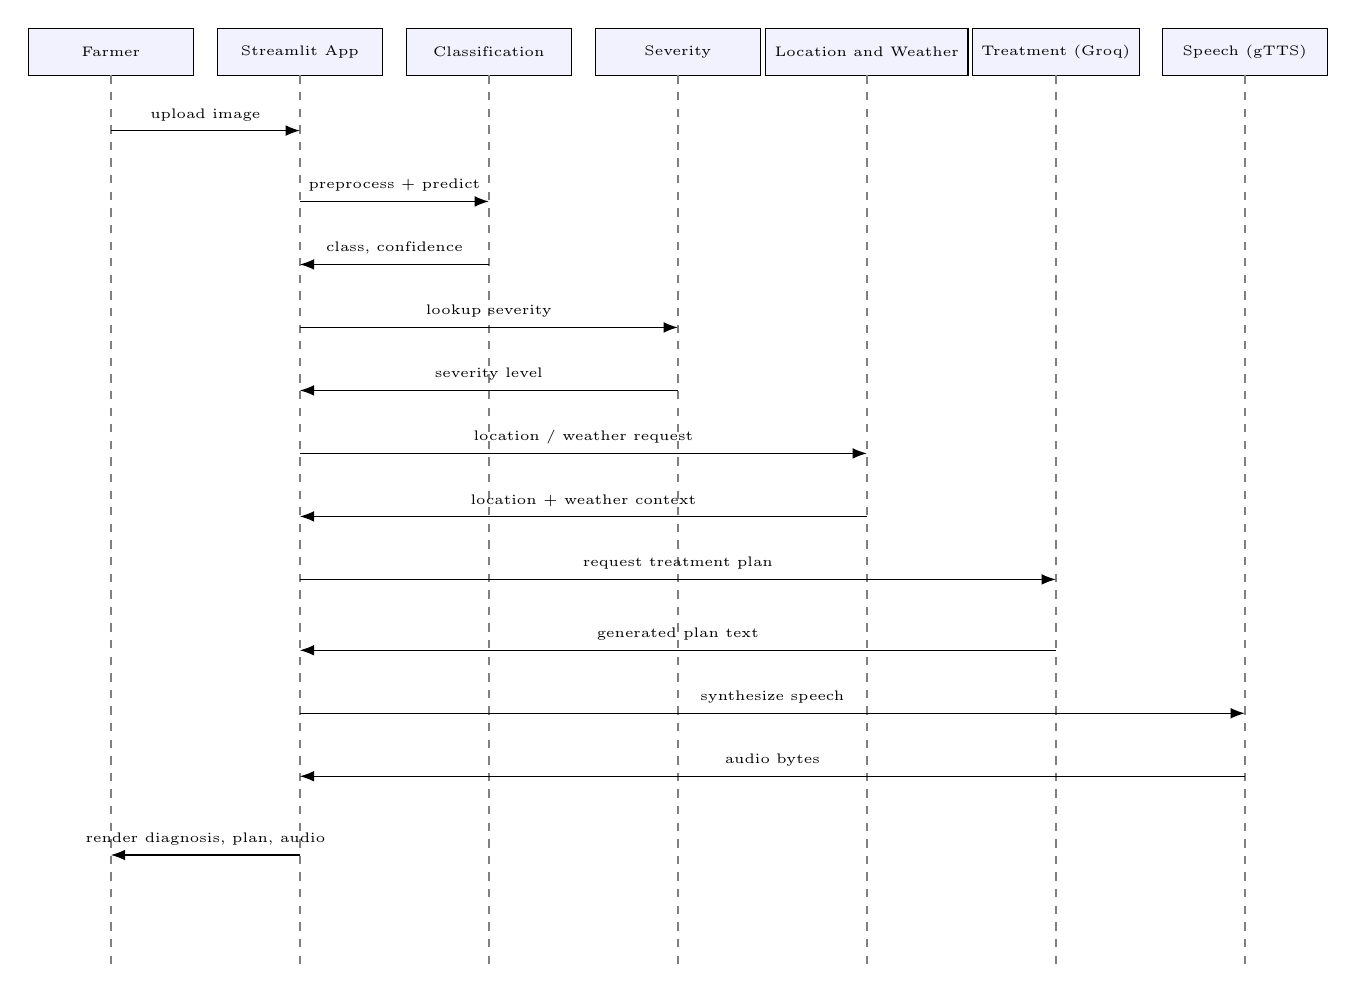
\begin{tikzpicture}[
  lifeline/.style={dashed, thick, gray},
  actorbox/.style={draw, minimum width=2.1cm, minimum height=0.6cm, align=center, font=\tiny, fill=blue!5},
  msg/.style={-{Latex[length=1.8mm]}, font=\tiny}
]
\foreach \x/\lbl in {0/Farmer, 2.4/Streamlit App, 4.8/Classification, 7.2/Severity, 9.6/Location and Weather, 12.0/Treatment (Groq), 14.4/Speech (gTTS)} {
  \node[actorbox] at (\x,0) {\lbl};
  \draw[lifeline] (\x,-0.3) -- (\x,-11.6);
}
\draw[msg] (0,-1.0) -- node[above]{upload image} (2.4,-1.0);
\draw[msg] (2.4,-1.9) -- node[above]{preprocess + predict} (4.8,-1.9);
\draw[msg] (4.8,-2.7) -- node[above]{class, confidence} (2.4,-2.7);
\draw[msg] (2.4,-3.5) -- node[above]{lookup severity} (7.2,-3.5);
\draw[msg] (7.2,-4.3) -- node[above]{severity level} (2.4,-4.3);
\draw[msg] (2.4,-5.1) -- node[above]{location / weather request} (9.6,-5.1);
\draw[msg] (9.6,-5.9) -- node[above]{location + weather context} (2.4,-5.9);
\draw[msg] (2.4,-6.7) -- node[above]{request treatment plan} (12.0,-6.7);
\draw[msg] (12.0,-7.6) -- node[above]{generated plan text} (2.4,-7.6);
\draw[msg] (2.4,-8.4) -- node[above]{synthesize speech} (14.4,-8.4);
\draw[msg] (14.4,-9.2) -- node[above]{audio bytes} (2.4,-9.2);
\draw[msg] (2.4,-10.2) -- node[above]{render diagnosis, plan, audio} (0,-10.2);
\end{tikzpicture}
\caption{Sequence diagram for a full upload-to-treatment-plan interaction.}
\label{fig:sequence}
\end{figure}

% ============================================================================
\chapter{Dataset and Model Development}
\label{ch:model}
% ============================================================================

This chapter documents the dataset, exploratory analysis, model architectures,
training methodology, and export pipeline exactly as carried out in the
project's training notebook. All figures, tables, and numbers in this chapter
are taken directly from an executed run of that notebook.

\section{Dataset Description}
The classification model is trained on the \textbf{PlantVillage} dataset,
obtained from Kaggle as \texttt{emmarex/plantdisease}~\cite{plantvillage-kaggle}.
The subset used for this project spans \textbf{15 classes} across three crops
-- Pepper (bell), Potato, and Tomato -- and contains 20{,}638 indexed leaf
images. Every image was verified with a full PIL integrity pass (0 unreadable
files found), and an exact-duplicate audit (byte-level MD5 hashing) removed
14 duplicate files (none of them cross-class), leaving \textbf{20{,}624 unique
images}.

\begin{table}[H]
\centering
\caption{Class distribution of the 15-class PlantVillage subset.}
\begin{tabular}{@{}lrr@{}}
\toprule
\textbf{Class} & \textbf{Images} & \textbf{Share} \\
\midrule
Tomato -- Tomato Yellow Leaf Curl Virus & 3{,}208 & 15.54\% \\
Tomato -- Bacterial spot & 2{,}127 & 10.31\% \\
Tomato -- Late blight & 1{,}909 & 9.25\% \\
Tomato -- Septoria leaf spot & 1{,}771 & 8.58\% \\
Tomato -- Spider mites (Two-spotted spider mite) & 1{,}676 & 8.12\% \\
Tomato -- healthy & 1{,}591 & 7.71\% \\
Pepper (bell) -- healthy & 1{,}478 & 7.16\% \\
Tomato -- Target Spot & 1{,}404 & 6.80\% \\
Potato -- Early blight & 1{,}000 & 4.85\% \\
Potato -- Late blight & 1{,}000 & 4.85\% \\
Tomato -- Early blight & 1{,}000 & 4.85\% \\
Pepper (bell) -- Bacterial spot & 997 & 4.83\% \\
Tomato -- Leaf Mold & 952 & 4.61\% \\
Tomato -- Tomato mosaic virus & 373 & 1.81\% \\
Potato -- healthy & 152 & 0.74\% \\
\midrule
\textbf{Total} & \textbf{20{,}638} & \textbf{100.00\%} \\
\bottomrule
\end{tabular}
\label{tab:classdist}
\end{table}

The largest class (Tomato Yellow Leaf Curl Virus, 3{,}208 images) is
\textbf{21.1$\times$} larger than the smallest (Potato healthy, 152 images) --
a real but moderate imbalance, addressed during training via class weighting
(Section~4.5).

\begin{figure}[H]
\centering
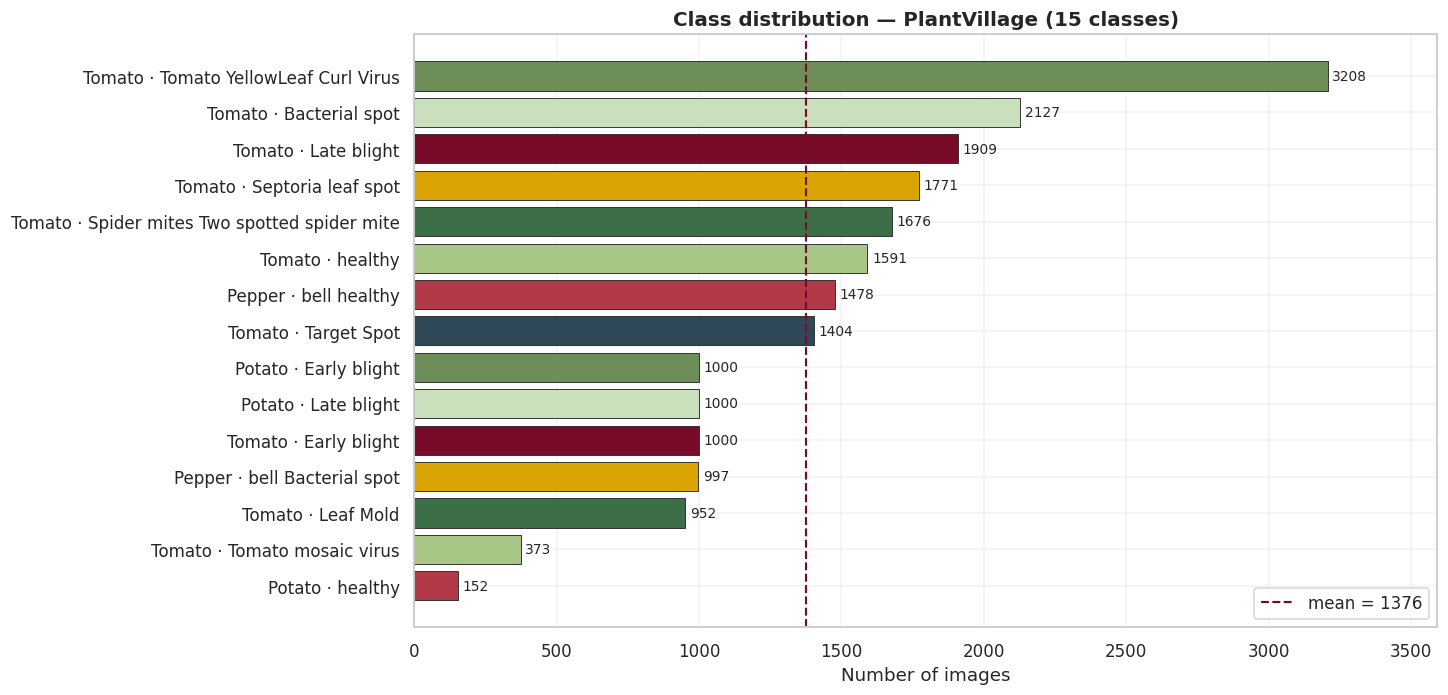
\includegraphics[width=0.92\textwidth]{01_class_distribution.png}
\caption{Class distribution across the 15-class PlantVillage subset.}
\label{fig:classdist}
\end{figure}

\begin{figure}[H]
\centering
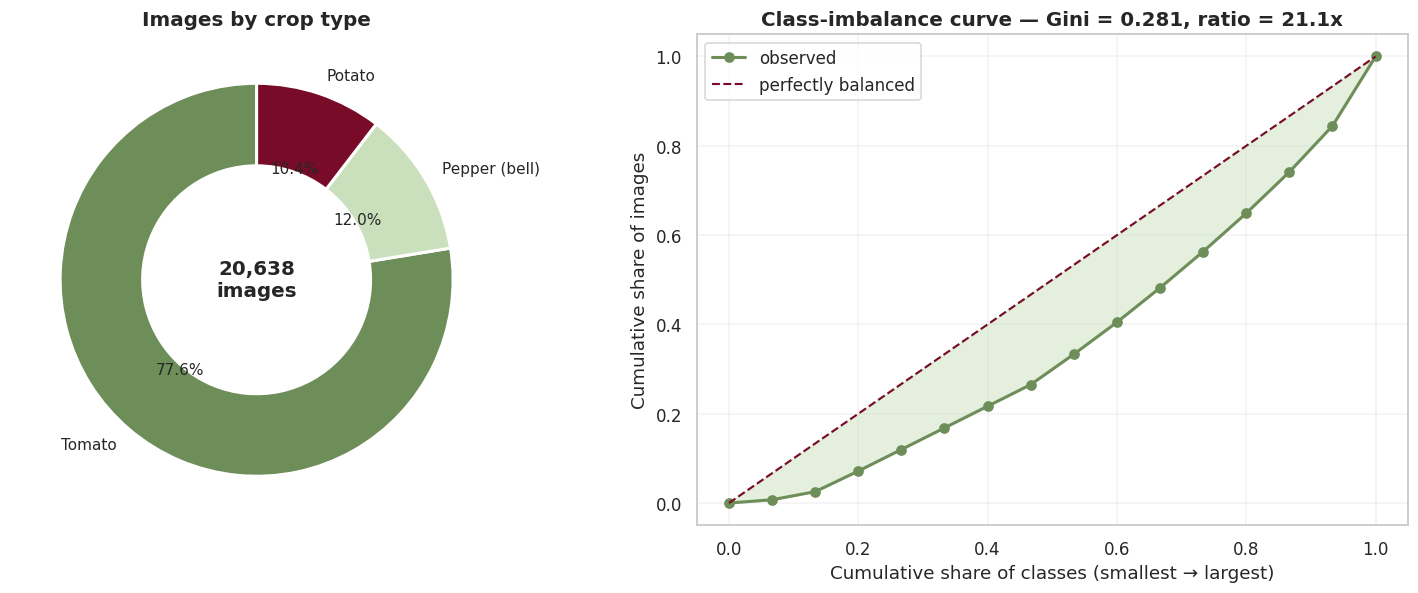
\includegraphics[width=0.92\textwidth]{02_imbalance_curve.png}
\caption{Image share by crop, and the class-imbalance (Lorenz) curve.}
\label{fig:imbalance}
\end{figure}

\section{Exploratory Data Analysis}
Before any model was built, the dataset was audited along six axes: class
balance, visual separability, resolution/file-size consistency, colour/brightness
signal, exact-duplicate leakage, and background consistency (a known shortcut
risk in PlantVillage, where a near-constant background could let a model learn
``lighting'' instead of ``disease'').

\begin{figure}[H]
\centering
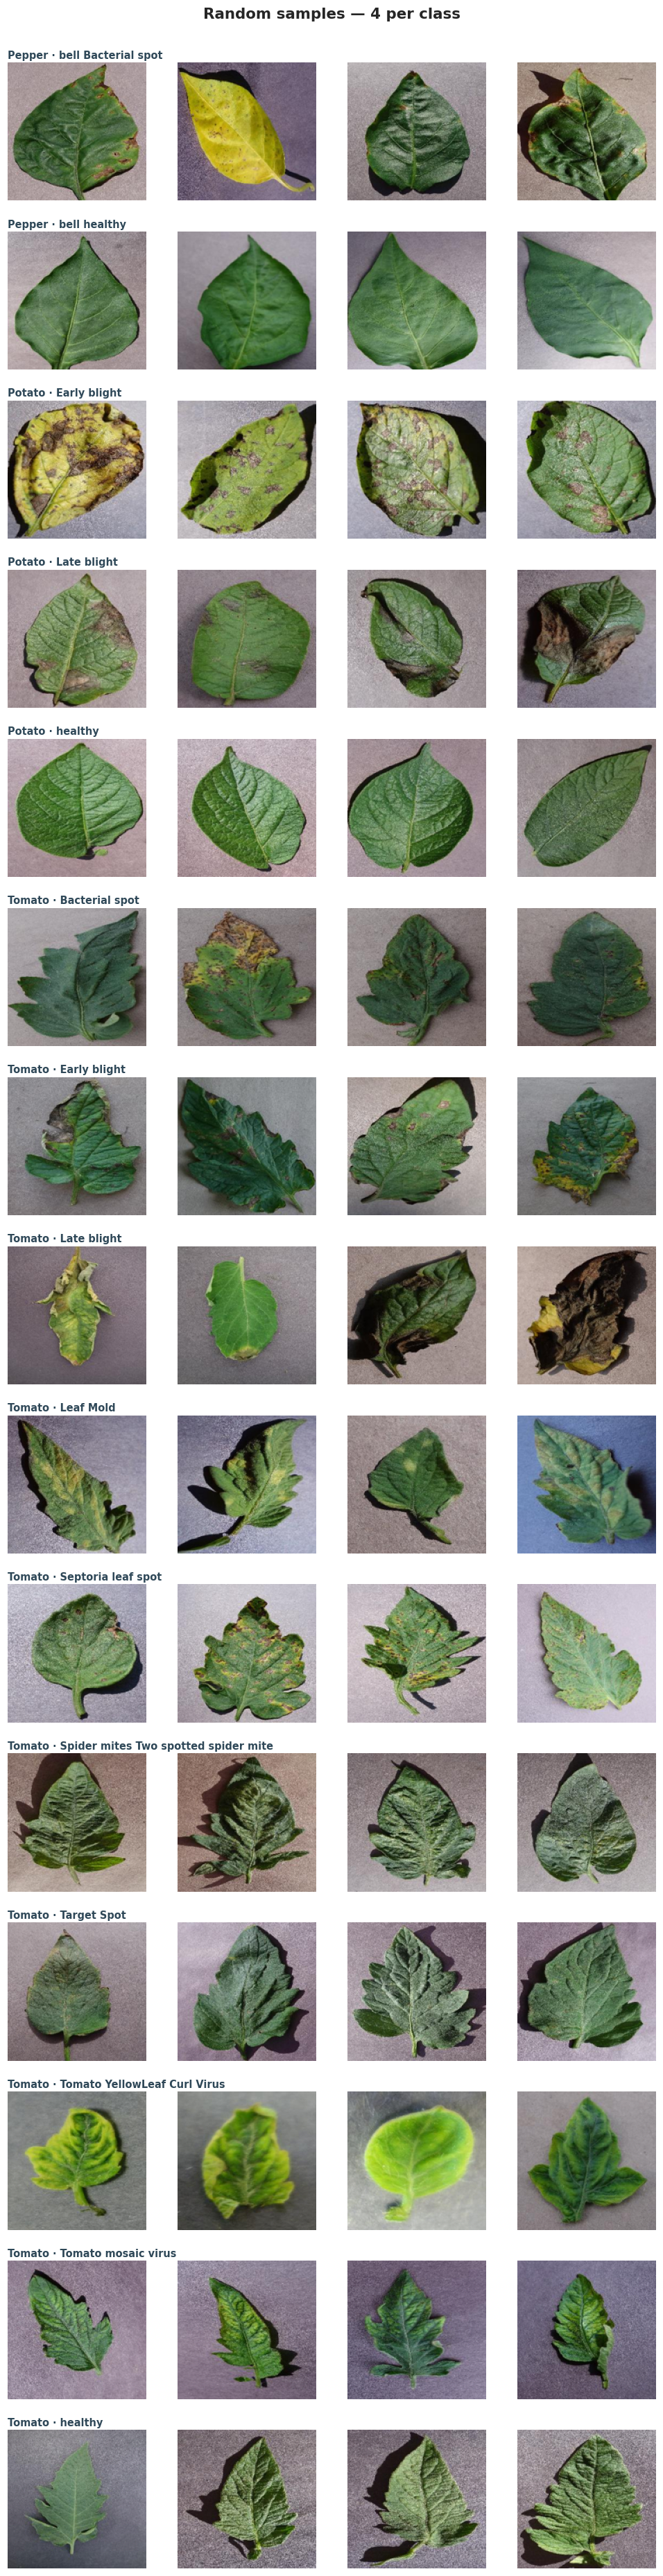
\includegraphics[width=0.95\textwidth]{03_sample_grid.png}
\caption{Random sample grid -- four images per class, as seen by the model.}
\label{fig:samplegrid}
\end{figure}

\begin{figure}[H]
\centering
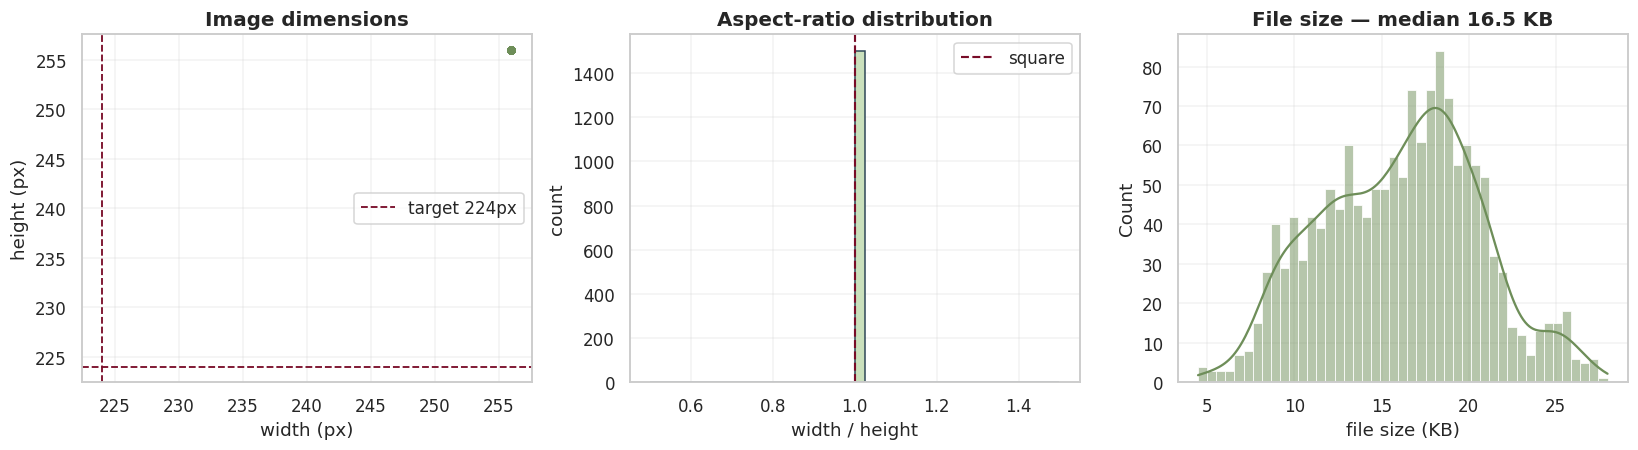
\includegraphics[width=0.92\textwidth]{04_resolution_filesize.png}
\caption{Resolution and file-size audit on a 1{,}500-image sample. PlantVillage
ships pre-cropped to a uniform 256$\times$256 resolution, so resizing to the
model's 224$\times$224 input costs almost nothing.}
\label{fig:resfilesize}
\end{figure}

\begin{figure}[H]
\centering
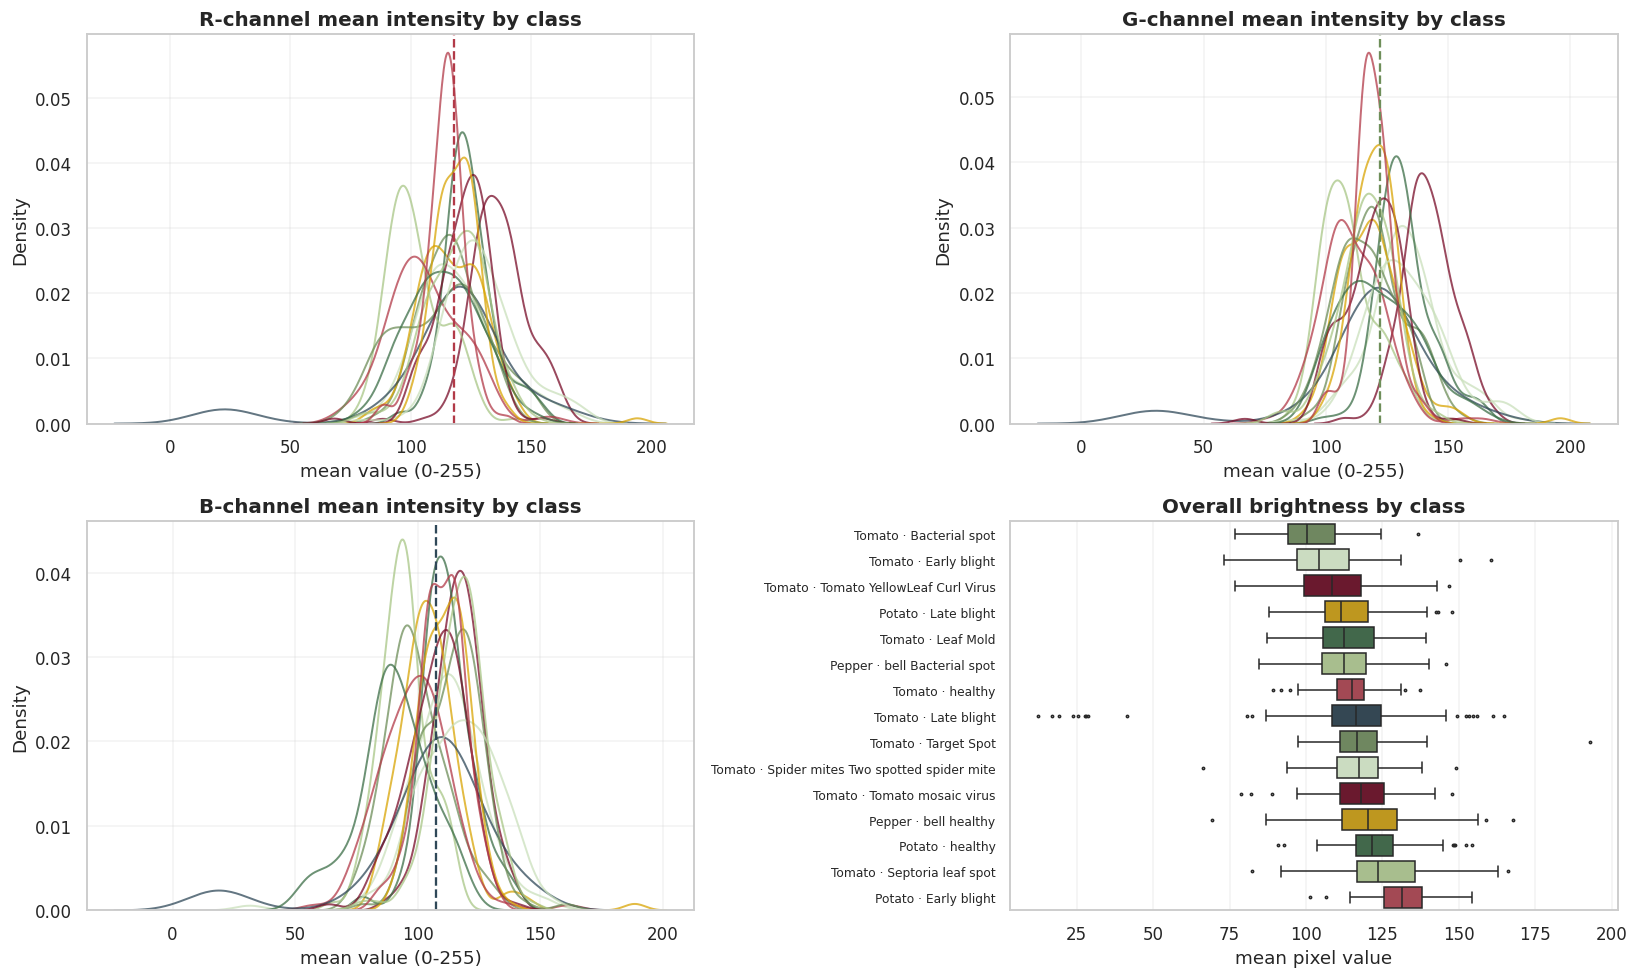
\includegraphics[width=0.92\textwidth]{05_colour_distributions.png}
\caption{Per-class colour and brightness distributions.}
\label{fig:colourdist}
\end{figure}

\begin{figure}[H]
\centering
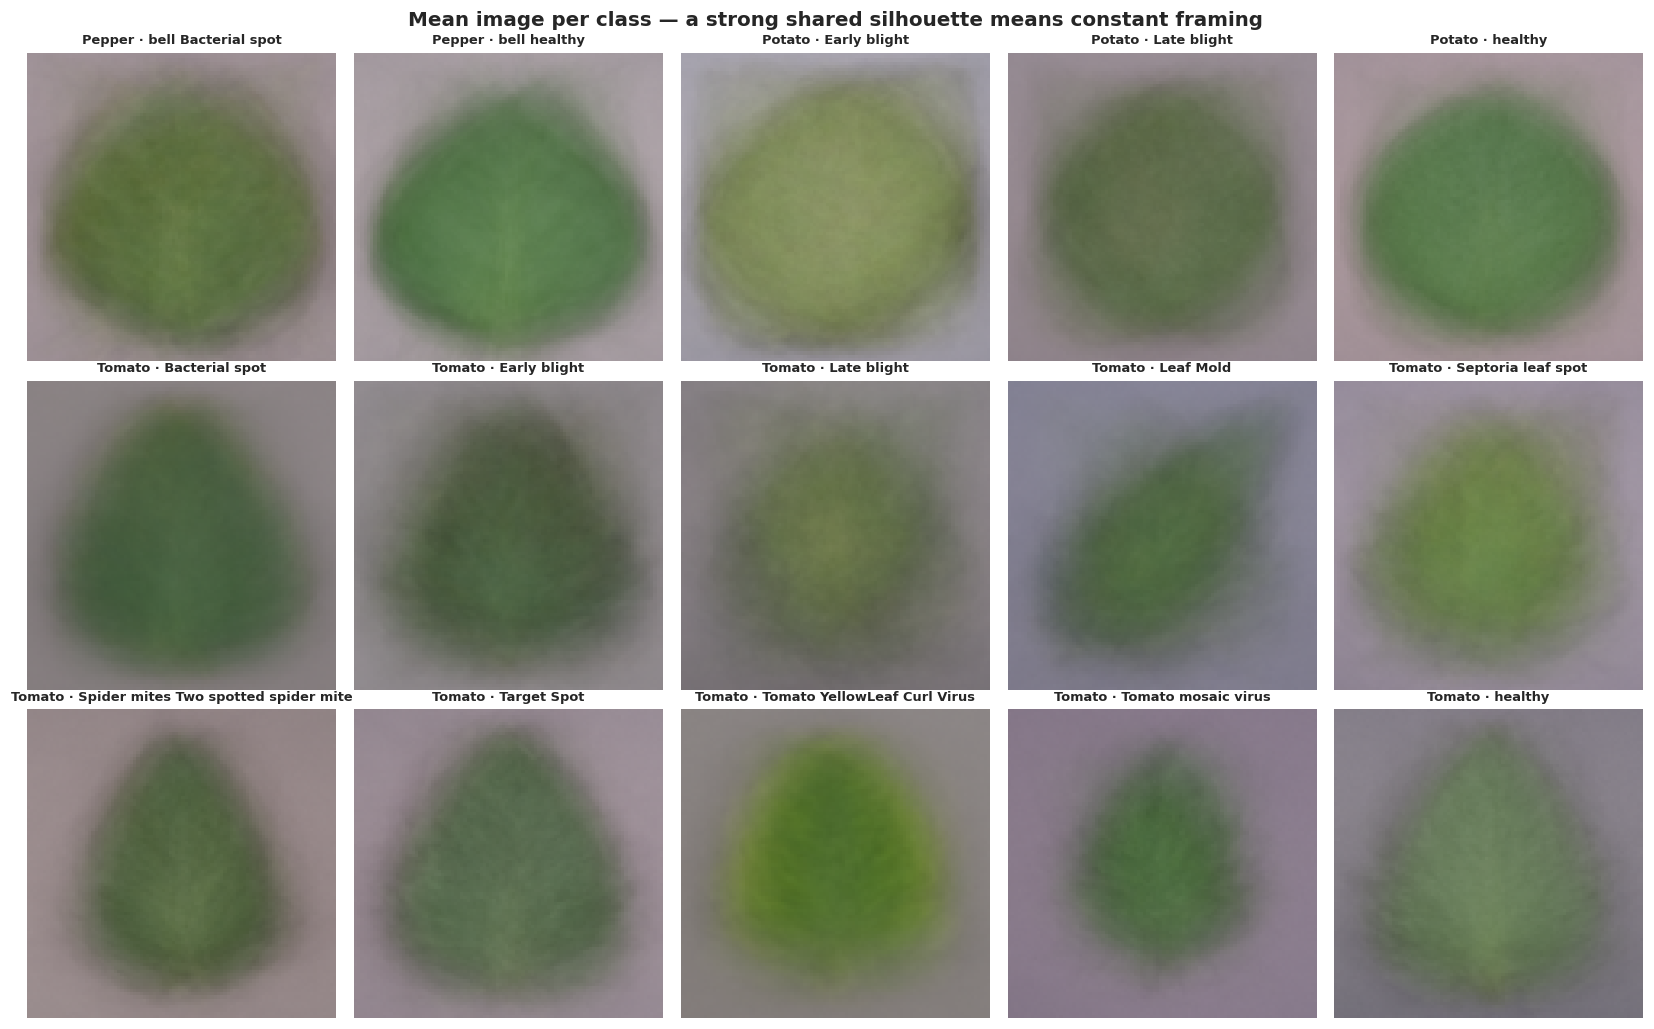
\includegraphics[width=0.85\textwidth]{06_mean_image_per_class.png}
\caption{Mean image per class. A strongly shared silhouette/background across
classes would indicate a shortcut the model could exploit instead of learning
the disease itself; the composition here is centred-leaf-on-grey-background
throughout, which is convenient for training but is also the specific reason
PlantVillage-trained models are known to generalize poorly to field photos
(Section~7.1).}
\label{fig:meanimage}
\end{figure}

\textbf{EDA takeaways:} imbalance is real but moderate (class weights enabled);
resolutions are uniform (no class is distorted more than another by resizing);
backgrounds are near-constant across the corpus; and only 0.07\% of images were
exact duplicates, none of them crossing class boundaries.

\section{Train / Validation / Test Split}
PlantVillage ships as one flat folder per class with no official split. A
\textbf{stratified} 70/15/15 split was constructed so every class keeps its
proportions in all three sets, with an explicit leakage check confirming zero
file overlap between splits.

\begin{table}[H]
\centering
\caption{Dataset split summary.}
\begin{tabular}{@{}lrr@{}}
\toprule
\textbf{Split} & \textbf{Images} & \textbf{Fraction} \\
\midrule
Train & 14{,}436 & 70.0\% \\
Validation & 3{,}094 & 15.0\% \\
Test & 3{,}094 & 15.0\% \\
\bottomrule
\end{tabular}
\label{tab:split}
\end{table}

The test set was touched exactly once, at the very end, and was never used
for any decision (model selection, early stopping, threshold tuning) during
development.

\begin{figure}[H]
\centering
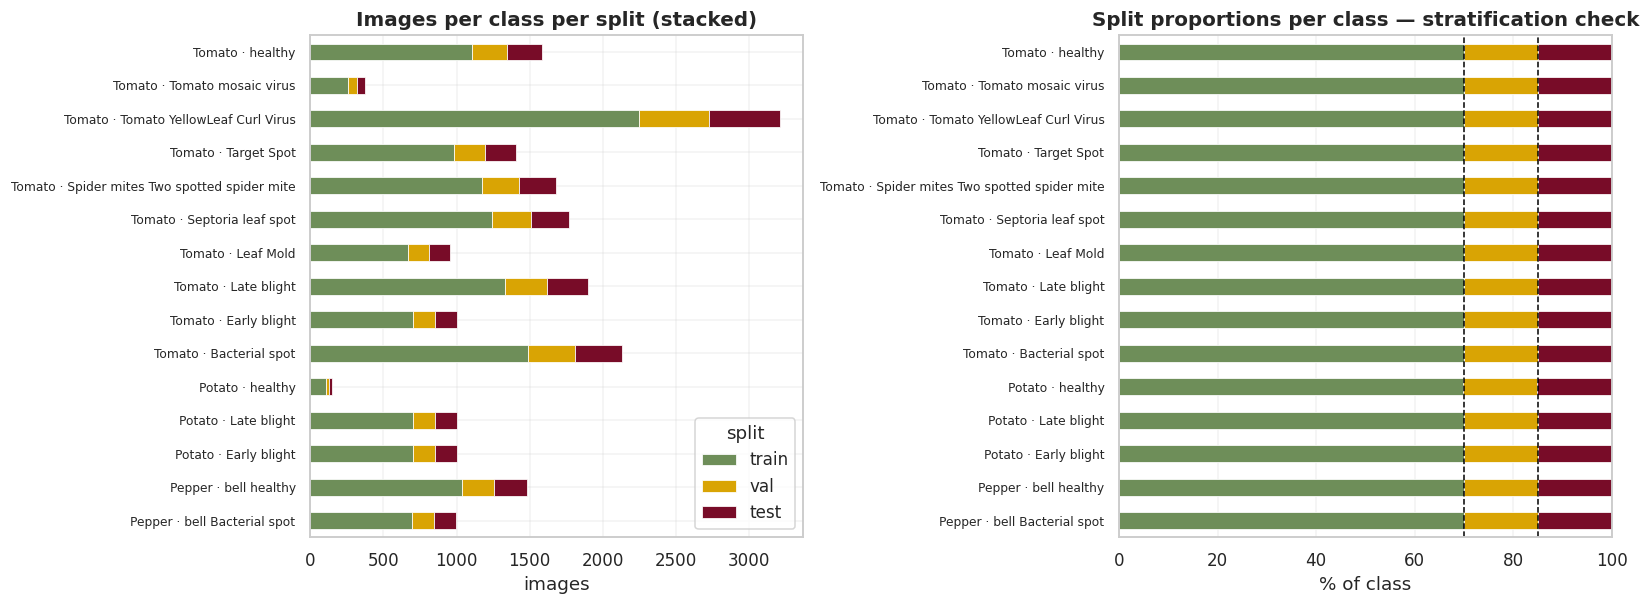
\includegraphics[width=0.92\textwidth]{07_split_distribution.png}
\caption{Images per class per split (stacked counts, and proportion).}
\label{fig:splitdist}
\end{figure}

\section{Input Pipeline and Data Augmentation}
Images are loaded and resized to $224\times224\times3$ through a
\texttt{tf.data} pipeline emitting raw \texttt{[0,255]} float tensors;
normalization is deliberately kept \emph{inside} each model (a
\texttt{Rescaling(1/255)} layer for the custom CNN, and EfficientNet's own
baked-in ImageNet normalization for Model~B) rather than in the pipeline, so
an exported model is self-contained and cannot be fed the wrong input range
downstream. Training images are augmented on the fly with:
\begin{itemize}[leftmargin=*]
    \item \texttt{RandomFlip} (horizontal and vertical)
    \item \texttt{RandomRotation} ($\pm$0.06 turns, $\approx\pm20^{\circ}$)
    \item \texttt{RandomZoom} (0.15)
    \item \texttt{RandomTranslation} (0.08, 0.08)
    \item \texttt{RandomContrast} (0.15)
    \item \texttt{RandomBrightness} (0.10, where supported)
\end{itemize}
With a batch size of 32, this yields 452 training batches, 97 validation
batches, and 97 test batches per epoch.

\begin{figure}[H]
\centering
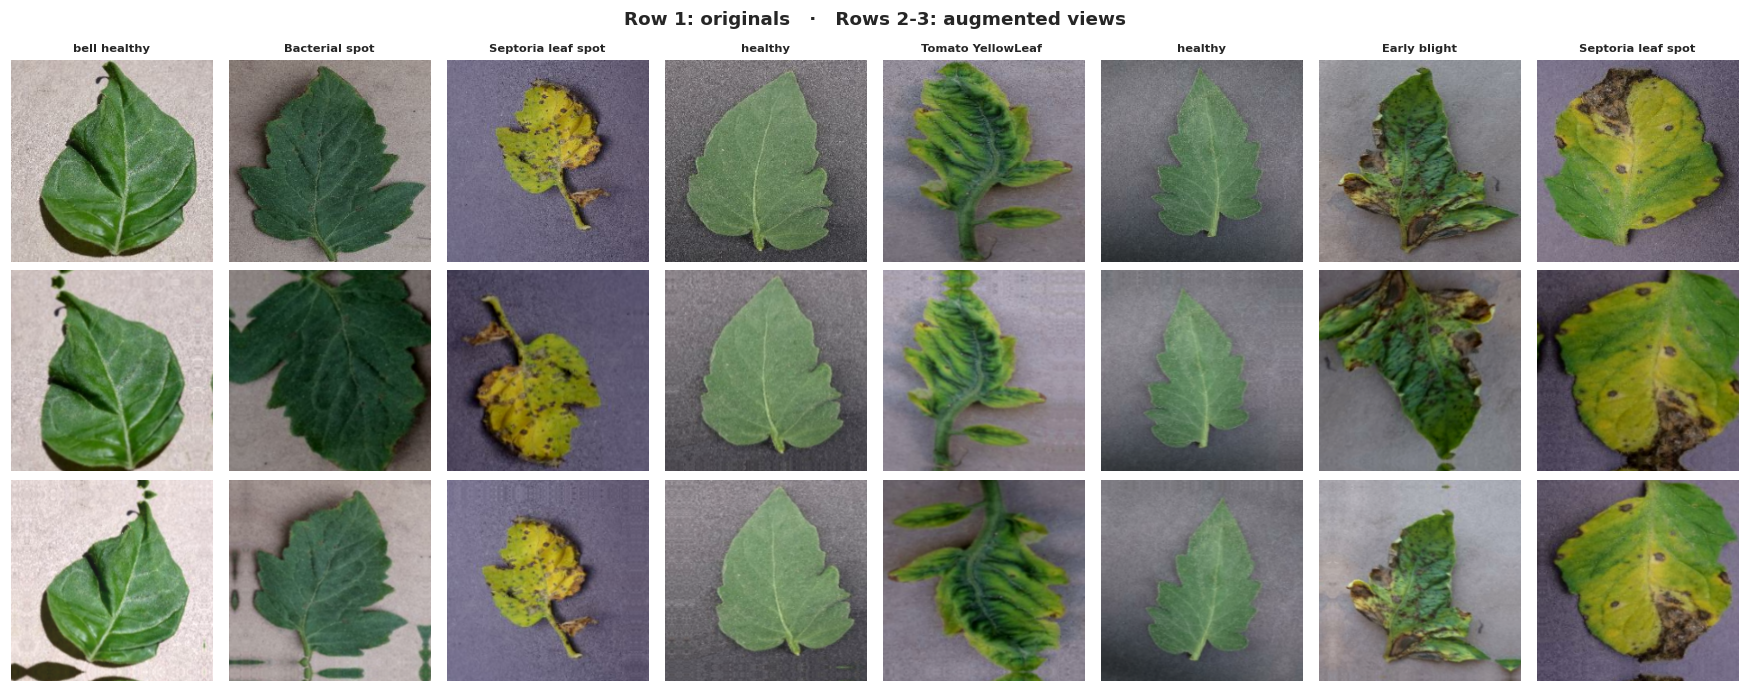
\includegraphics[width=0.92\textwidth]{08_augmentation_preview.png}
\caption{Augmentation sanity check -- row 1: originals; rows 2--3: augmented
views. Labels remain visually legible after augmentation.}
\label{fig:augpreview}
\end{figure}

\section{Class Imbalance Handling}
Because the largest class outnumbers the smallest by 21.1$\times$, per-class
weights (``balanced'' scheme, scikit-learn) were computed and applied during
training so rare classes contribute proportionally more to the training
gradient. Potato -- healthy (106 training images) receives the largest weight
(9.079); Tomato -- Tomato Yellow Leaf Curl Virus (2{,}245 training images)
receives the smallest (0.429).

\section{Model Architectures}

\subsection{Model A -- Custom CNN (trained from scratch)}
A VGG-style convolutional network: six blocks of two $3\times3$ convolutions
followed by batch normalization and $2\times2$ max-pooling, with channel
widths $64 \rightarrow 128 \rightarrow 128 \rightarrow 256 \rightarrow 512
\rightarrow 512$, followed by a dense classifier head.

\begin{table}[H]
\centering
\caption{Custom CNN architecture summary (10.90M total parameters, 41.60~MB).}
\begin{tabular}{@{}lll@{}}
\toprule
\textbf{Stage} & \textbf{Layers} & \textbf{Output shape} \\
\midrule
Input & -- & $224\times224\times3$ \\
Rescale & \texttt{Rescaling(1/255)} & $224\times224\times3$ \\
Block 1--6 & [Conv2D $\times$2, BatchNorm, MaxPool2D(2)] $\times$6, & \\
& widths 64/128/128/256/512/512 & $7\times7\times512$ \\
Classifier & Flatten $\to$ Dense(256, ReLU) $\to$ Dense(64, ReLU) & \\
& $\to$ Dropout(0.3) $\to$ Dense(15, Softmax) & 15 \\
\bottomrule
\end{tabular}
\label{tab:cnnarch}
\end{table}

\lstinputlisting[language=Python, caption={Custom CNN definition and compilation (excerpted from the training notebook).}, label={lst:cnn}]{listings/build_scratch_cnn.py}

\subsection{Model B -- EfficientNetB3 (transfer learning)}
An ImageNet-pretrained EfficientNetB3~\cite{tan2019efficientnet} backbone
(\texttt{include\_top=False}, global max pooling) with a lightweight custom
head, trained in two stages: first with the backbone entirely frozen (head-only
training), then with the top 60 backbone layers unfrozen for fine-tuning
(BatchNorm layers kept frozen throughout to preserve pretrained statistics).

\begin{table}[H]
\centering
\caption{EfficientNetB3 architecture summary (11.18M total parameters, 42.65~MB).}
\begin{tabular}{@{}lll@{}}
\toprule
\textbf{Stage} & \textbf{Layers} & \textbf{Output shape} \\
\midrule
Input & -- & $224\times224\times3$ \\
Backbone & EfficientNetB3 (386 layers, ImageNet weights, pooling=max) & 1536 \\
Head & Dense(256, ReLU) $\to$ Dropout(0.3) $\to$ Dense(15, Softmax) & 15 \\
\bottomrule
\end{tabular}
\label{tab:effnetarch}
\end{table}

\lstinputlisting[language=Python, caption={EfficientNetB3 model definition (excerpted from the training notebook).}, label={lst:effnet}]{listings/build_efficientnet.py}

\section{Training Configuration}
Both models were compiled with the Adamax optimizer and categorical
cross-entropy loss with label smoothing (0.05), tracked with categorical
accuracy and top-3 categorical accuracy. Training used early stopping
(patience 6, restoring the best weights), a learning-rate-on-plateau schedule
(halving on stagnation, floor $10^{-7}$), model checkpointing, and CSV logging.

\begin{table}[H]
\centering
\caption{Training hyperparameters (\texttt{CFG} block, training notebook).}
\begin{tabular}{@{}ll@{}}
\toprule
\textbf{Parameter} & \textbf{Value} \\
\midrule
Image size & $224\times224\times3$ \\
Batch size & 32 \\
Validation / test fraction & 15\% / 15\% (stratified) \\
Random seed & 42 \\
Epochs -- Custom CNN & 30 (max) \\
Epochs -- EfficientNet head & 8 \\
Epochs -- EfficientNet fine-tune & 7 \\
Learning rate -- Custom CNN & $1\times10^{-3}$ (Adamax) \\
Learning rate -- EfficientNet head & $1\times10^{-3}$ (Adamax) \\
Learning rate -- EfficientNet fine-tune & $1\times10^{-5}$ (Adamax) \\
Fine-tune layers unfrozen (from top) & 60 \\
Early-stopping patience & 6 epochs \\
Class weighting & Enabled (``balanced'') \\
Label smoothing & 0.05 \\
\bottomrule
\end{tabular}
\label{tab:hyperparams}
\end{table}

In practice, the Custom CNN ran for \textbf{25 of its 30 maximum epochs}
before early stopping triggered, restoring weights from epoch~19
(112.3 minutes total). EfficientNetB3 completed its full schedule: 8 epochs of
head-only training followed by 7 epochs of fine-tuning (60.6 minutes total,
both stages combined), with the best fine-tuning weights taken from the final
(7th) fine-tuning epoch.

\begin{figure}[H]
\centering
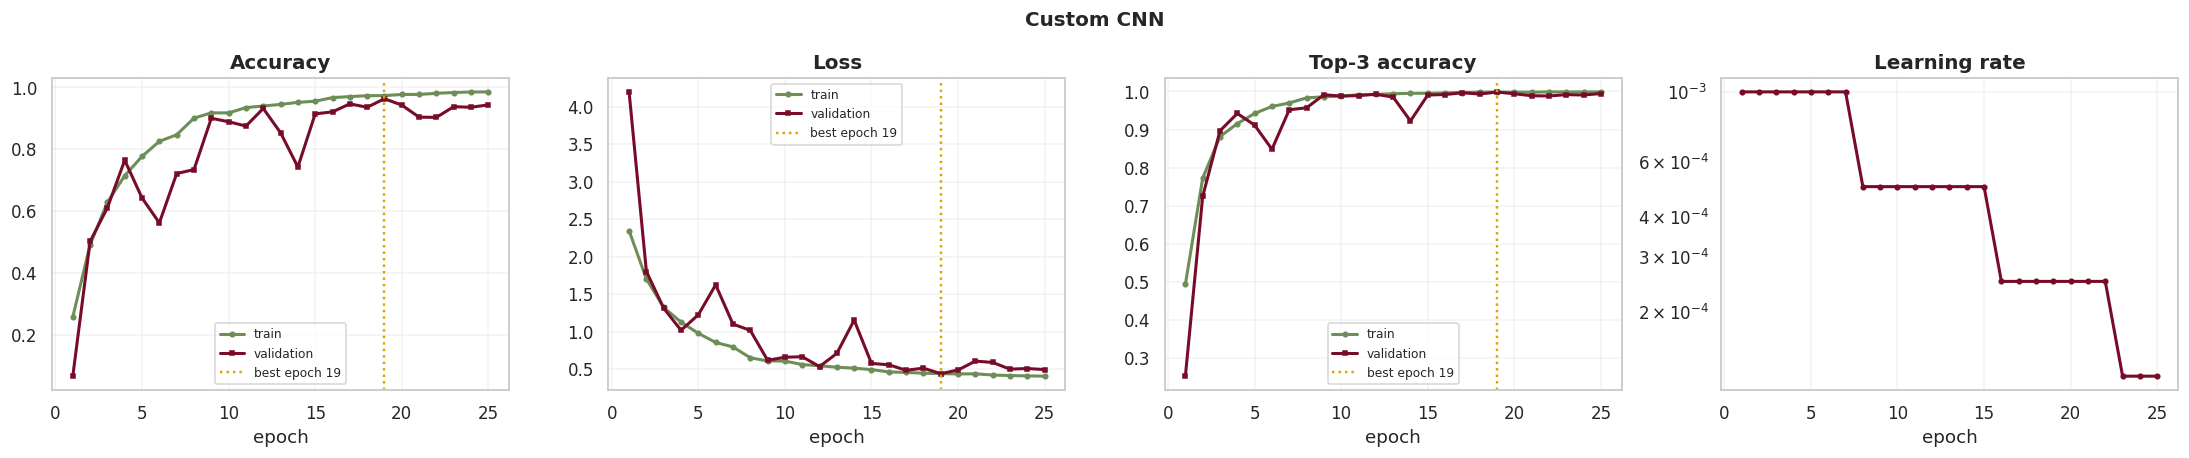
\includegraphics[width=0.92\textwidth]{09_curves_custom_cnn.png}
\caption{Custom CNN learning curves. Final train/validation accuracy gap:
+4.20 percentage points (mild overfitting).}
\label{fig:curvescnn}
\end{figure}

\begin{figure}[H]
\centering
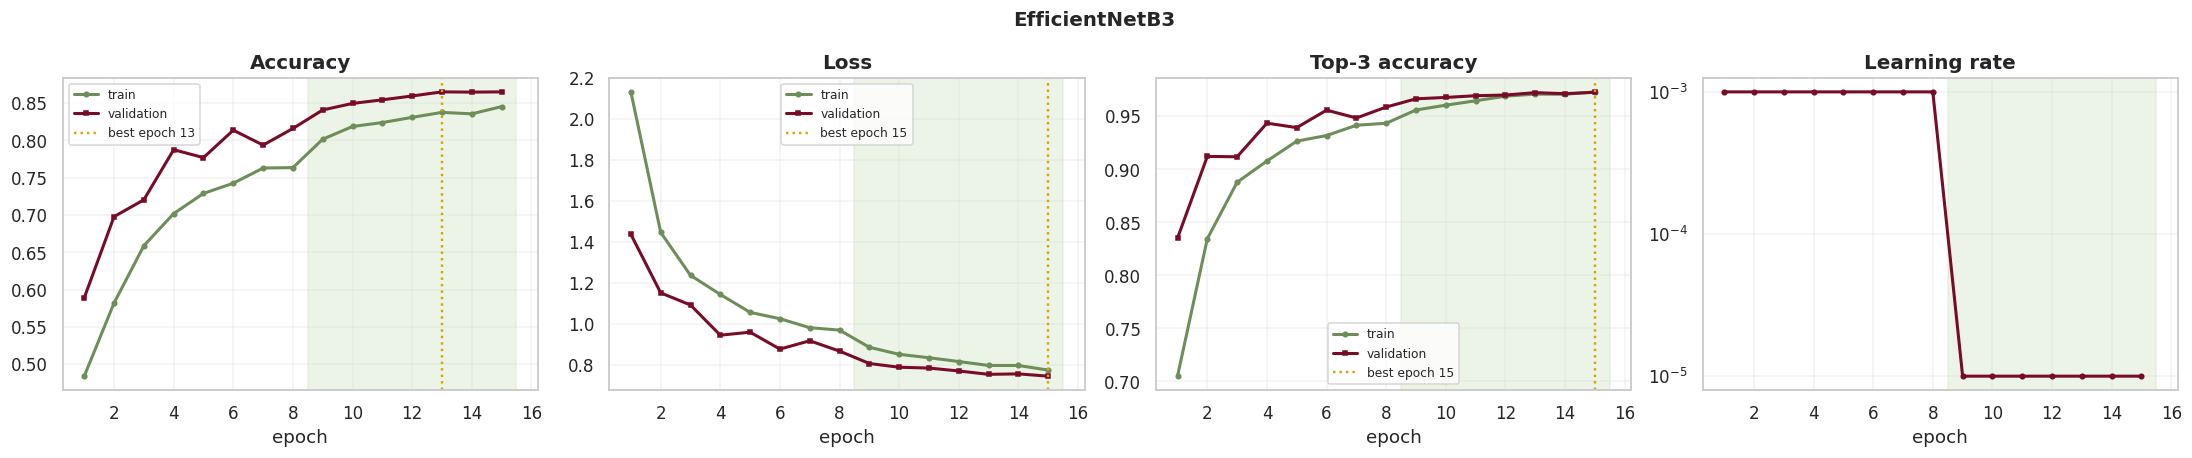
\includegraphics[width=0.92\textwidth]{09_curves_efficientnetb3.png}
\caption{EfficientNetB3 learning curves (shaded region = fine-tuning stage).
Final train/validation accuracy gap: $-$1.98 percentage points (healthy fit,
no sign of overfitting).}
\label{fig:curveseffnet}
\end{figure}

\section{Model Export and Deployment Packaging}
The chosen model (selection criterion: Section~6.2) was exported to three
formats to serve three different needs: \texttt{.keras} (native, for further
training), \texttt{.h5} (legacy/portability), and \texttt{TFLite} (for
lightweight/on-device inference), the latter in both fp32 and fp16-quantized
variants. Every exported artifact was re-run on real test images and checked
for prediction agreement against the source Keras model before being reported
as usable -- a converted model that \emph{runs} is not automatically a
converted model that is \emph{correct}. TFLite fidelity and latency results
are reported in Section~6.9.

\lstinputlisting[language=Python, caption={Deployment-shaped TFLite inference wrapper (excerpted from the training notebook) -- this mirrors what a server or mobile client actually runs.}, label={lst:tflite}]{listings/tflite_classifier.py}

% ============================================================================
\chapter{Implementation}
% ============================================================================

\section{Development Environment}
The application is implemented in Python and served with Streamlit. Secrets
(API keys for the LLM provider, etc.) are loaded from a local \texttt{.env}
file via \texttt{python-dotenv} and never committed to source control.
Logging is enabled at \texttt{INFO} level to trace request timings (e.g.
prediction latency) during development.

\section{Application Workflow}
The application exposes three top-level tabs -- \emph{Home}, \emph{About},
and \emph{Disease Recognition} -- implemented as a segmented top navigation
bar rather than a sidebar page picker. The \emph{Disease Recognition} tab
drives the primary workflow:
\begin{enumerate}[leftmargin=*]
    \item The user uploads a leaf photograph (JPG/JPEG/PNG).
    \item The image is preprocessed (resized, normalized) and passed to the
    trained classification model (Chapter~4), returning a predicted class and
    confidence score.
    \item A fresh prediction invalidates any previously generated severity,
    location, weather, treatment plan, or audio held in session state, so
    stale results are never shown alongside a new diagnosis.
    \item The severity engine (Section~5.3) computes a severity level for the
    predicted condition.
    \item If the plant is not healthy, the user is prompted for their
    location (GPS or manual), current weather is fetched for that location,
    and a treatment plan is generated on request (Section~5.4).
    \item At each stage, an audio narration of the result can be generated
    on demand (Section~5.7).
\end{enumerate}
Switching the interface language at any point clears cached results that were
generated in the previous language, so text and audio never mix languages
within a single displayed result.

\section{Severity Assessment}
Severity is computed from a lookup table of plant-pathology facts for each
diagnosed condition -- pathogen type (fungal / bacterial / viral / oomycete /
pest), whether the condition is curable, its spread rate, and its yield
impact -- combined into a severity score and level. This is a deliberate
design choice: severity is a property of the \emph{disease}, not of how
confident a particular model run happened to be, so the same diagnosis always
receives the same severity, and severity remains meaningful even when model
confidence is comparatively low.

\section{Localized Treatment Recommendation}
Given the predicted crop and condition, the computed severity, and the
farmer's resolved location, the treatment engine calls a hosted large
language model (Groq's \texttt{llama-3.3-70b-versatile}) to produce a
treatment plan tailored to the region -- climate-appropriate advice, locally
available products, and timing -- in the farmer's selected language. Location
is resolved either from a manually typed place name (forward-geocoded) or
from browser GPS coordinates (reverse-geocoded), both via the OpenStreetMap
Nominatim API, which requires no API key.

\section{Weather Context}
Treatment plans are conditioned on real weather rather than generic seasonal
advice. The weather engine calls Open-Meteo's forecast endpoint once per
resolved location, retrieving daily aggregates (max/min temperature,
precipitation, cloud cover, humidity) for yesterday, today, and tomorrow in a
single request. Open-Meteo was chosen because it is free and keyless for
non-commercial use, unlike alternatives that require a paid subscription for
equivalent day-summary data.

\section{Text-to-Speech Output}
Both the diagnosis summary and the treatment plan can be converted to spoken
audio via gTTS, a free, keyless wrapper around Google's text-to-speech
endpoint whose language codes map directly onto the application's Hindi/English
language keys. Markdown formatting and emoji are stripped from the text before
synthesis so that the reader does not attempt to vocalize symbols. A
server-side engine was chosen over the browser's native speech-synthesis API
because it produces consistent audio regardless of the visiting device or
browser's installed voices -- a real concern for Hindi, which many
browsers/operating systems do not ship a voice for at all.

\section{Multilingual Interface}
Every user-facing string is resolved through a single translation function
keyed by the active language, which is read from and written to Streamlit's
session state. This centralizes all UI text in one place and makes the
language toggle a simple session-state write rather than a page reload.

\section{User Interface}
The interface layers a restrained, translucent-material visual design on top
of Streamlit's default theme: blurred/translucent surfaces for cards and the
sidebar, a segmented-control style for the tab bar and radio toggles, subtle
press feedback on buttons (scale-down on press, no bounce on release), and
typography tuned per heading level (tracking and line-height), implemented
entirely via scoped CSS injected into the page, with a reduced-motion media
query that disables transitions for users who request it.

% ============================================================================
\chapter{Results and Output Screens}
% ============================================================================

\section{Evaluation Metrics}
Accuracy alone is misleading on an imbalanced dataset (Section~4.5), so the
notebook reports a broader set of metrics on the held-out, never-touched test
set of 3{,}094 images:

\begin{table}[H]
\centering
\caption{Evaluation metrics and their purpose.}
\begin{tabular}{@{}ll@{}}
\toprule
\textbf{Metric} & \textbf{Why it is reported} \\
\midrule
Accuracy & Headline number, but flattered by class imbalance \\
Balanced accuracy & Mean per-class recall -- the honest accuracy here \\
Macro-F1 & Treats a 152-image class as equal to a 3{,}208-image one \\
Weighted-F1 & Reflects the population a deployed model would actually meet \\
Top-3 accuracy & Relevant for a UI that could surface top candidates \\
Cohen's $\kappa$ / MCC & Chance-corrected agreement; MCC is robust under skew \\
ROC-AUC / PR-AUC (OvR) & Threshold-free ranking quality \\
\bottomrule
\end{tabular}
\end{table}

\section{Quantitative Results}
\begin{table}[H]
\centering
\caption{Test-set results (3{,}094 held-out images), Custom CNN vs.\ EfficientNetB3.}
\begin{tabular}{@{}lrr@{}}
\toprule
\textbf{Metric} & \textbf{Custom CNN} & \textbf{EfficientNetB3} \\
\midrule
Accuracy & \textbf{95.51\%} & 87.10\% \\
Balanced accuracy & \textbf{94.86\%} & 88.06\% \\
Precision (macro) & \textbf{94.88\%} & 86.66\% \\
Recall (macro) & 94.86\% & \textbf{88.06\%} \\
F1 (macro) & \textbf{94.59\%} & 86.92\% \\
Precision (weighted) & \textbf{95.80\%} & 88.09\% \\
Recall (weighted) & \textbf{95.51\%} & 87.10\% \\
F1 (weighted) & \textbf{95.52\%} & 87.12\% \\
Top-3 accuracy & \textbf{99.81\%} & 97.41\% \\
Cohen's $\kappa$ & \textbf{0.9509} & 0.8594 \\
MCC & \textbf{0.9511} & 0.8605 \\
Log-loss (lower is better) & \textbf{0.1663} & 0.4437 \\
ROC-AUC (macro) & \textbf{0.9992} & 0.9932 \\
PR-AUC (macro) & \textbf{0.9907} & 0.9460 \\
Mean confidence & 0.9237 & 0.7933 \\
Inference time (3{,}094 images, GPU) & 11.45 s & 26.26 s \\
Inference time per image & \textbf{3.70 ms} & 8.49 ms \\
Total training time & 112.3 min & 60.6 min \\
\bottomrule
\end{tabular}
\label{tab:results}
\end{table}

\noindent \textbf{Model selection.} By macro-F1 -- the metric least flattered
by class imbalance -- the Custom CNN outperforms EfficientNetB3 (94.59\% vs.\
86.92\%) and was selected as the deployment model. This is a somewhat
counter-intuitive result: the smaller, from-scratch model beats ImageNet
transfer learning here, plausibly because PlantVillage's controlled,
lab-uniform images (Section~4.2) reduce the advantage that ImageNet-pretrained
low-level features normally provide, while the deeper custom architecture (6
conv blocks vs.\ a frozen/lightly-fine-tuned backbone) can fit the
in-distribution training signal more closely.

\begin{figure}[H]
\centering
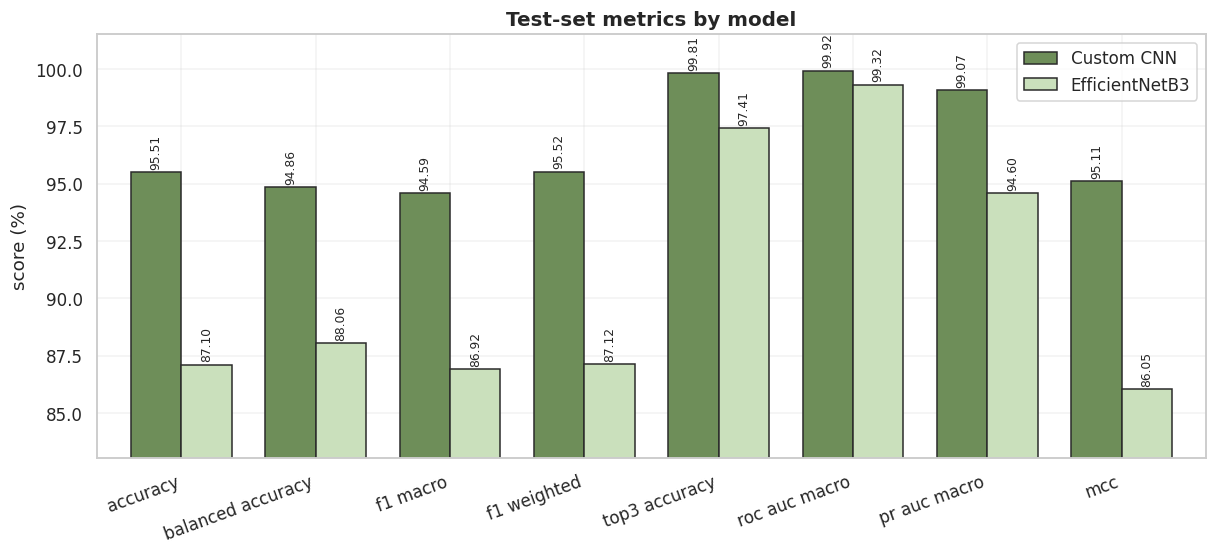
\includegraphics[width=0.92\textwidth]{10_metric_comparison.png}
\caption{Test-set metric comparison across both models.}
\label{fig:metriccompare}
\end{figure}

\section{Confusion Analysis}
\begin{figure}[H]
\centering
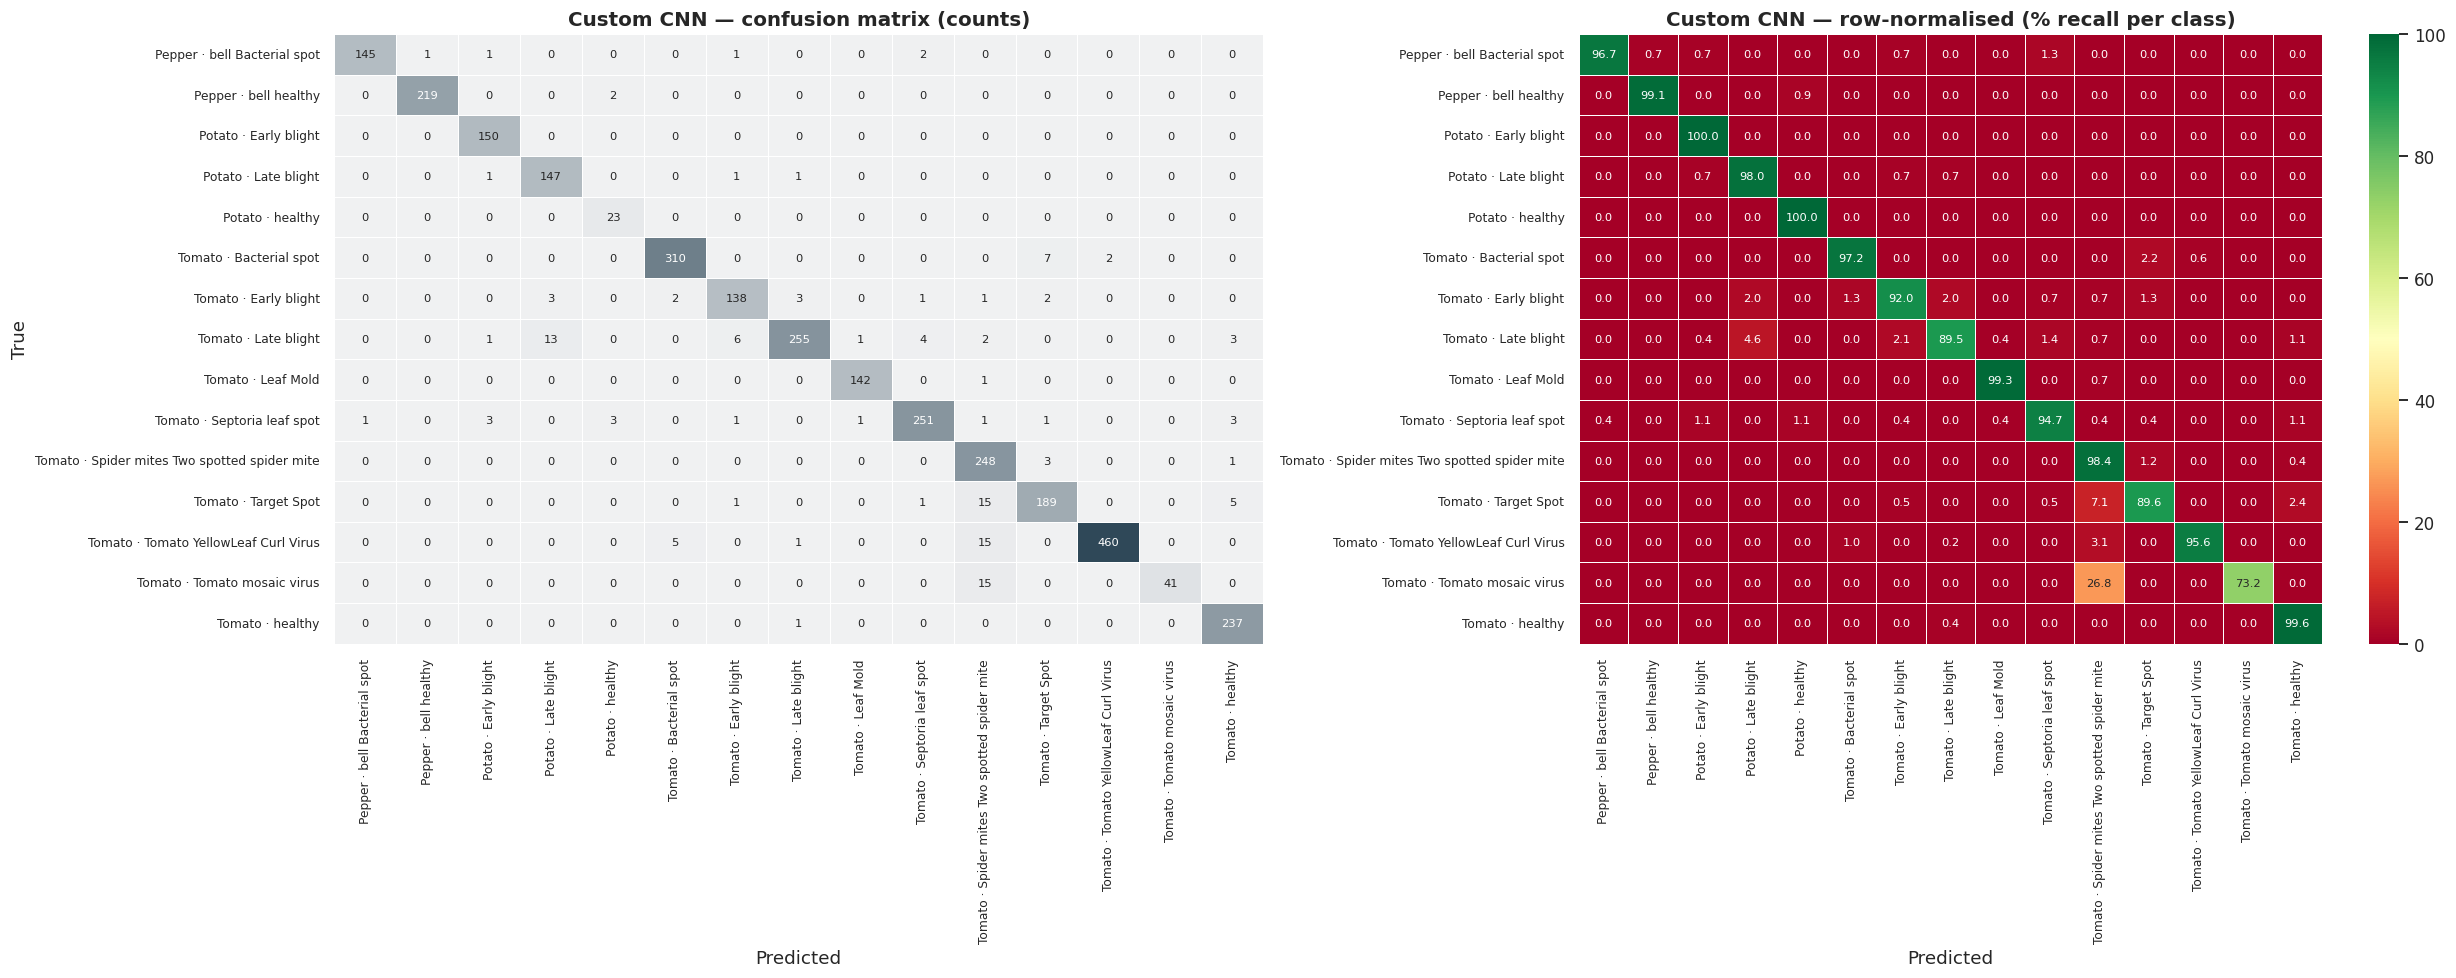
\includegraphics[width=0.98\textwidth]{11_confusion_custom_cnn.png}
\caption{Confusion matrix, Custom CNN (counts and row-normalized \%).}
\label{fig:confcnn}
\end{figure}

\begin{figure}[H]
\centering
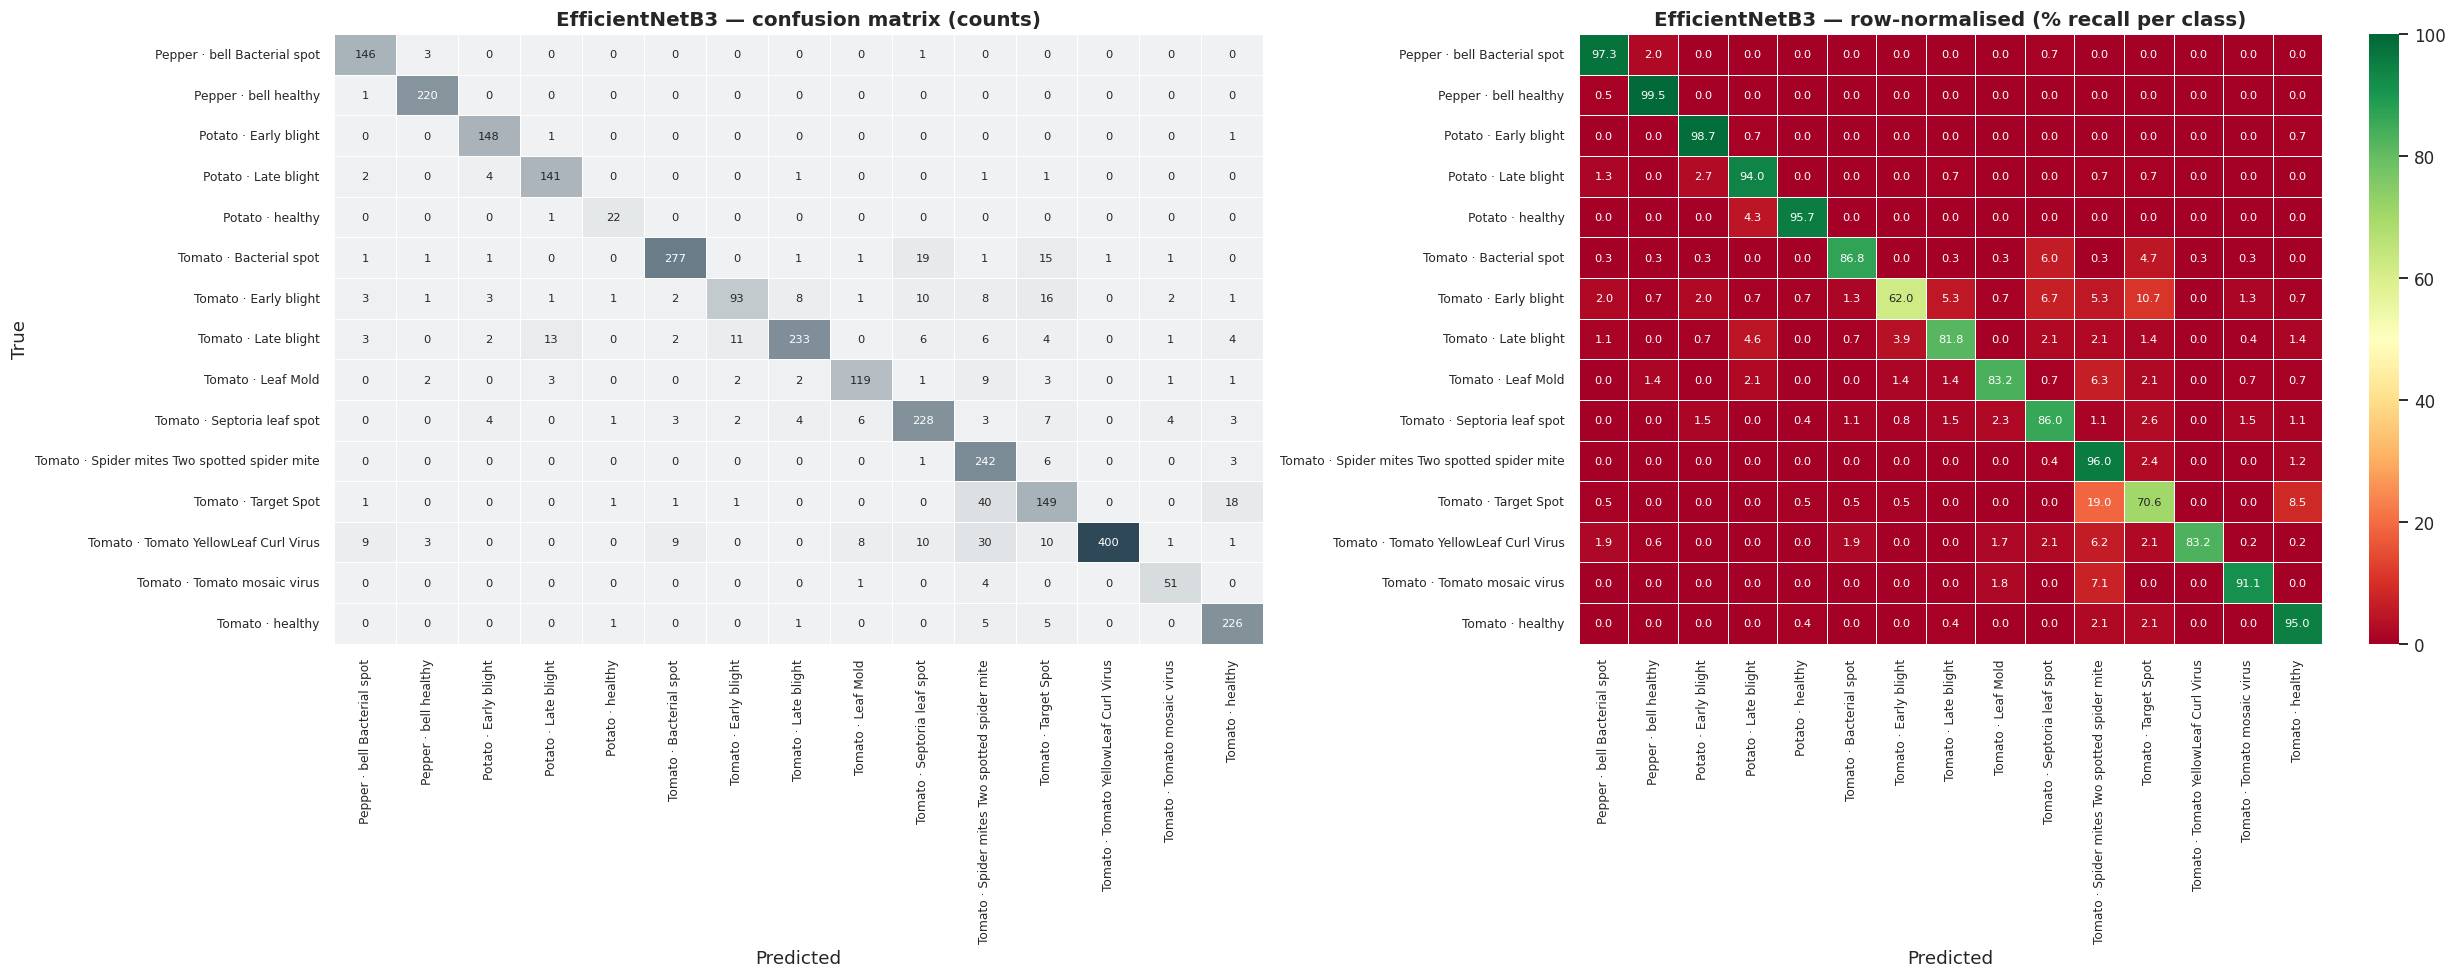
\includegraphics[width=0.98\textwidth]{11_confusion_efficientnetb3.png}
\caption{Confusion matrix, EfficientNetB3 (counts and row-normalized \%).}
\label{fig:confeffnet}
\end{figure}

\begin{table}[H]
\centering
\caption{Most frequent confusions, Custom CNN (test set).}
\begin{tabular}{@{}rll@{}}
\toprule
\textbf{Count} & \textbf{True class} & \textbf{Predicted as} \\
\midrule
15 & Tomato -- Tomato mosaic virus & Tomato -- Spider mites \\
15 & Tomato -- Target Spot & Tomato -- Spider mites \\
15 & Tomato -- Tomato Yellow Leaf Curl Virus & Tomato -- Spider mites \\
13 & Tomato -- Late blight & Potato -- Late blight \\
7 & Tomato -- Bacterial spot & Tomato -- Target Spot \\
6 & Tomato -- Late blight & Tomato -- Early blight \\
\bottomrule
\end{tabular}
\end{table}

Almost every confusion is between visually similar tomato conditions, or
between the two crops' late-blight classes (which are caused by related
oomycete pathogens and can look similar on a leaf) -- consistent with the
model learning genuine visual disease features rather than an unrelated
shortcut.

\section{Per-Class Performance}
\begin{table}[H]
\centering
\caption{Per-class precision, recall, and F1 -- Custom CNN (test set, 3{,}094 images).}
\begin{tabular}{@{}lrrrr@{}}
\toprule
\textbf{Class} & \textbf{Precision} & \textbf{Recall} & \textbf{F1} & \textbf{Support} \\
\midrule
Pepper -- Bacterial spot & 0.9932 & 0.9667 & 0.9797 & 150 \\
Pepper -- healthy & 0.9955 & 0.9910 & 0.9932 & 221 \\
Potato -- Early blight & 0.9615 & 1.0000 & 0.9804 & 150 \\
Potato -- Late blight & 0.9018 & 0.9800 & 0.9393 & 150 \\
Potato -- healthy & 0.8214 & 1.0000 & 0.9020 & 23 \\
Tomato -- Bacterial spot & 0.9779 & 0.9718 & 0.9748 & 319 \\
Tomato -- Early blight & 0.9324 & 0.9200 & 0.9262 & 150 \\
Tomato -- Late blight & 0.9770 & 0.8947 & 0.9341 & 285 \\
Tomato -- Leaf Mold & 0.9861 & 0.9930 & 0.9895 & 143 \\
Tomato -- Septoria leaf spot & 0.9691 & 0.9472 & 0.9580 & 265 \\
Tomato -- Spider mites & 0.8322 & 0.9841 & 0.9018 & 252 \\
Tomato -- Target Spot & 0.9356 & 0.8957 & 0.9153 & 211 \\
Tomato -- Yellow Leaf Curl Virus & 0.9957 & 0.9563 & 0.9756 & 481 \\
Tomato -- mosaic virus & 1.0000 & 0.7321 & 0.8454 & 56 \\
Tomato -- healthy & 0.9518 & 0.9958 & 0.9733 & 238 \\
\midrule
\textbf{Accuracy} & \multicolumn{3}{c}{0.9551} & 3{,}094 \\
\textbf{Macro avg} & 0.9488 & 0.9486 & 0.9459 & 3{,}094 \\
\textbf{Weighted avg} & 0.9580 & 0.9551 & 0.9552 & 3{,}094 \\
\bottomrule
\end{tabular}
\label{tab:perclass}
\end{table}

The weakest class by F1 is Tomato -- mosaic virus (0.8454), driven by low
recall (0.7321, i.e.\ it is the class most often \emph{missed}) despite
perfect precision -- consistent with it being the rarest class in the training
set (261 images) even after class weighting.

\begin{figure}[H]
\centering
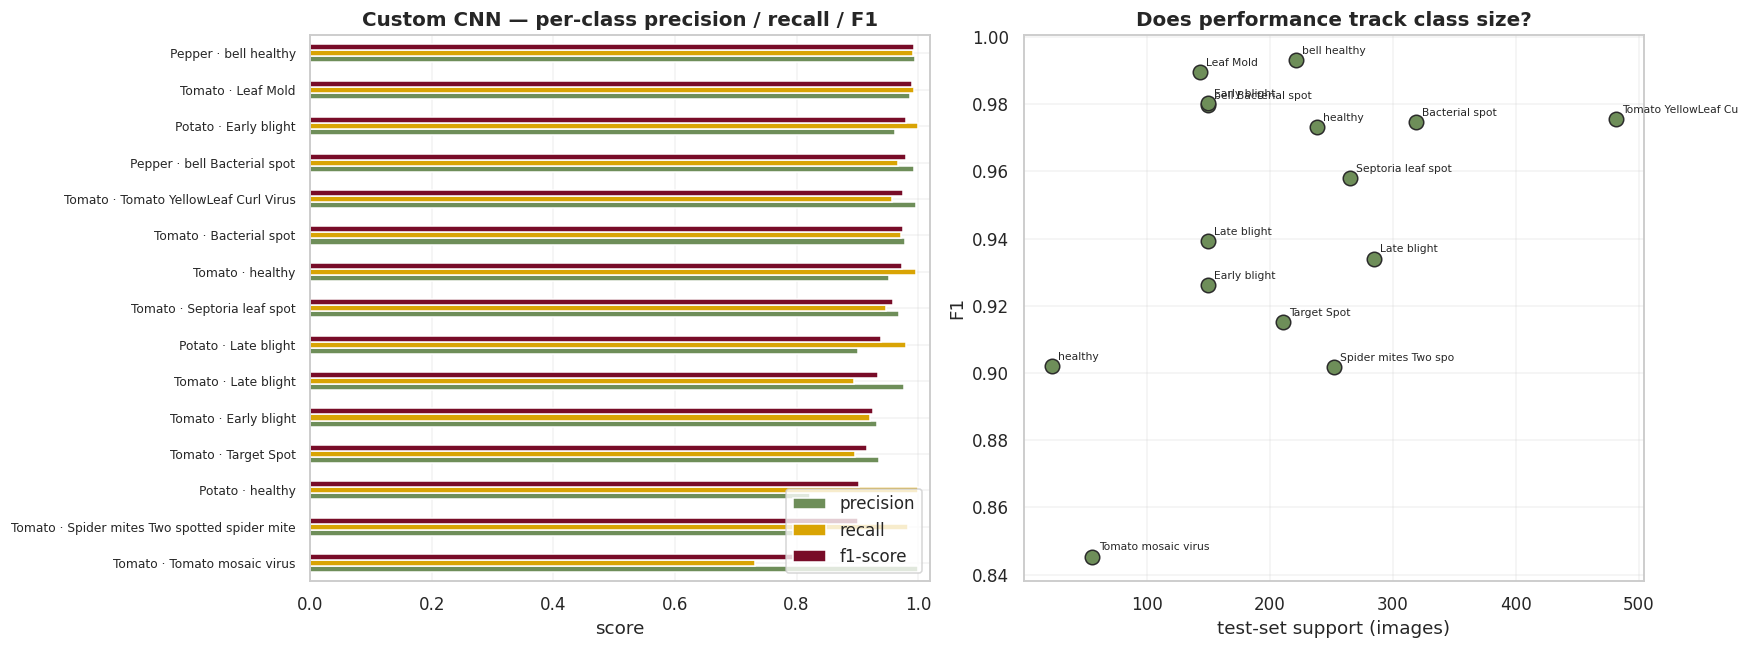
\includegraphics[width=0.92\textwidth]{12_per_class_metrics.png}
\caption{Per-class precision, recall, and F1 -- Custom CNN.}
\label{fig:perclassfig}
\end{figure}

\section{ROC and Precision--Recall Curves}
\begin{figure}[H]
\centering
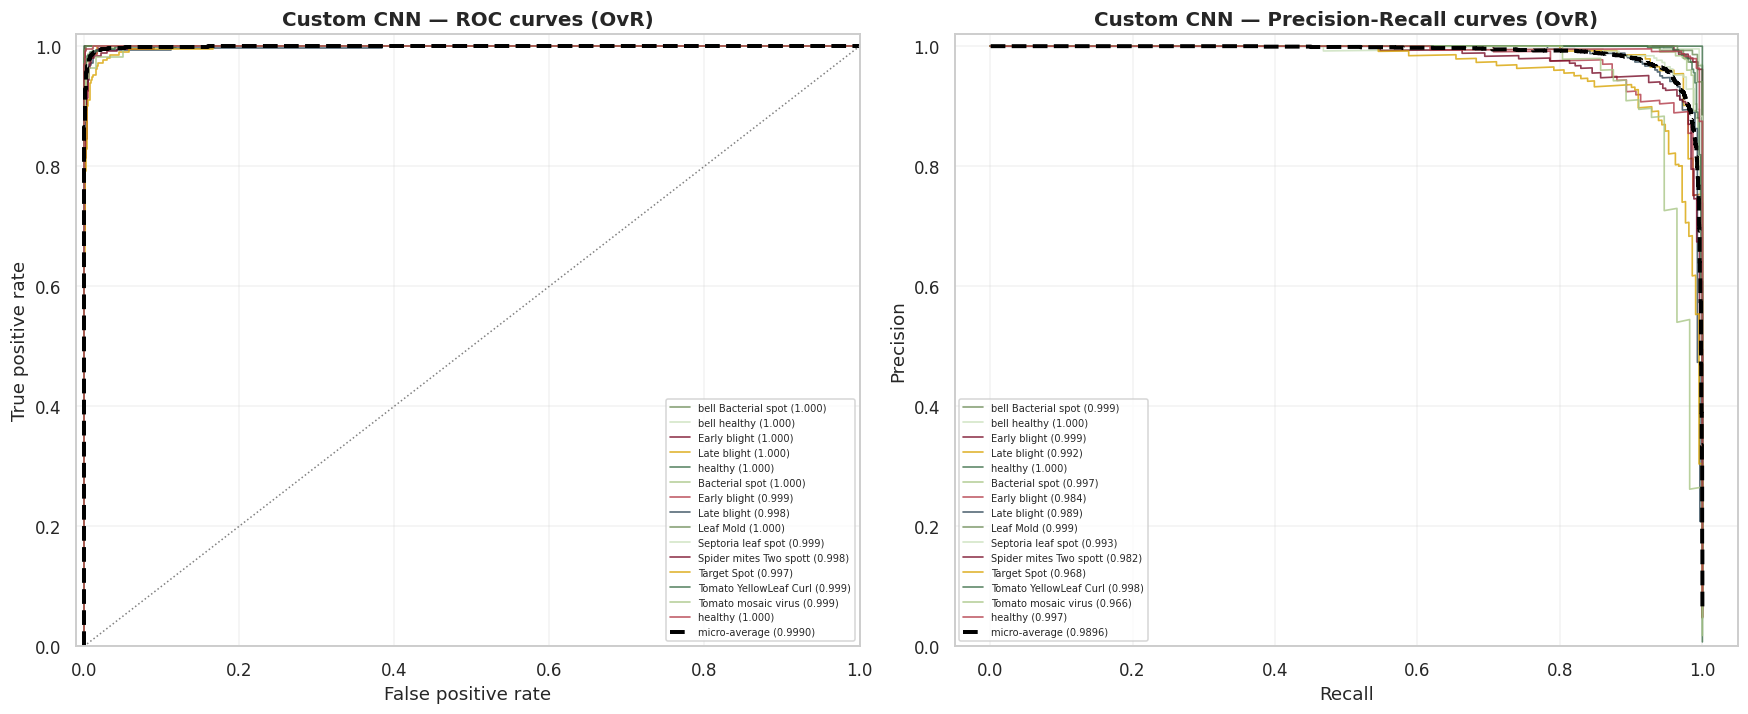
\includegraphics[width=0.98\textwidth]{13_roc_pr_curves.png}
\caption{One-vs-rest ROC and Precision--Recall curves, Custom CNN. Micro-average
ROC-AUC $=0.9990$.}
\label{fig:rocpr}
\end{figure}

\section{Confidence Calibration}
\begin{figure}[H]
\centering
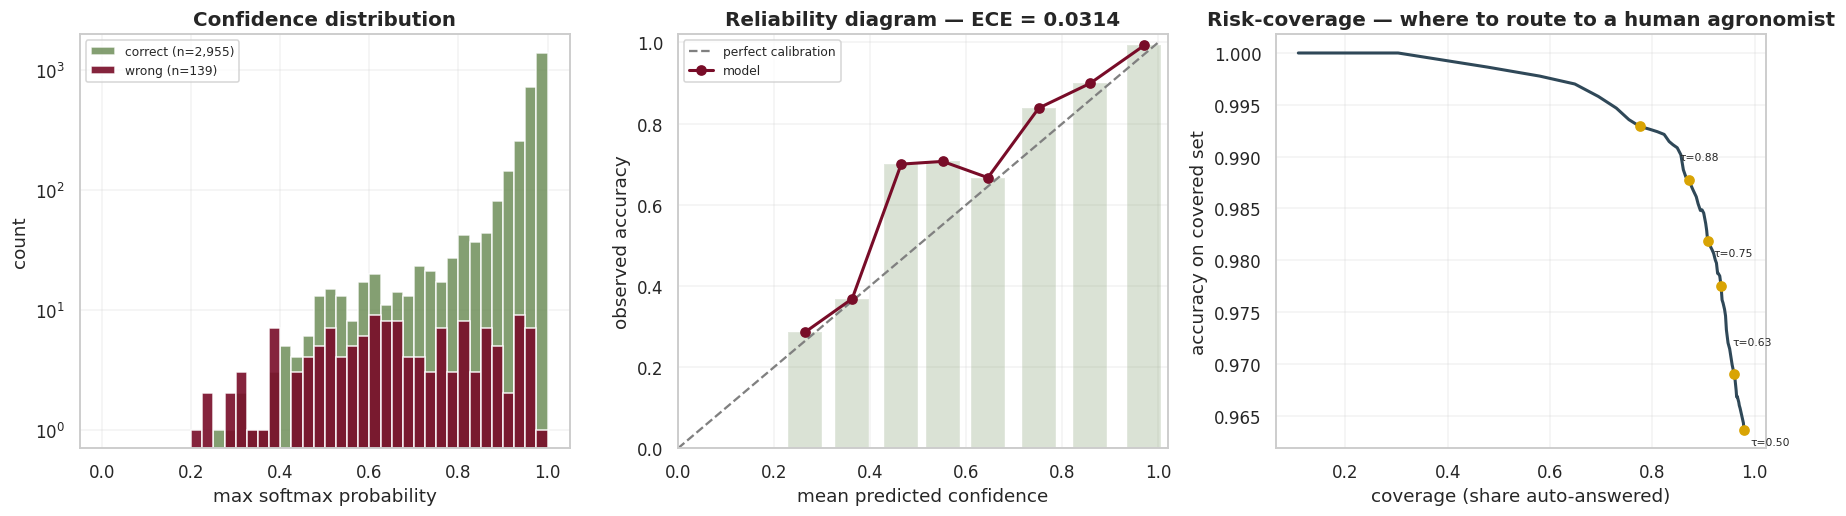
\includegraphics[width=0.98\textwidth]{14_confidence_calibration.png}
\caption{Confidence distribution and calibration, Custom CNN.}
\label{fig:calibration}
\end{figure}

The model's Expected Calibration Error is \textbf{0.0314} (generally
considered acceptable, i.e.\ $<0.05$, for a user-facing confidence display),
with a mean confidence of \textbf{0.936} on correct predictions versus
\textbf{0.664} on incorrect ones. This separation is large enough to support
a practical safety measure: a confidence threshold below which the
application should say ``diagnosis unclear -- try another photo'' rather than
present a low-confidence label as if it were certain (discussed further in
Section~7.1).

\section{Error Analysis}
\begin{figure}[H]
\centering
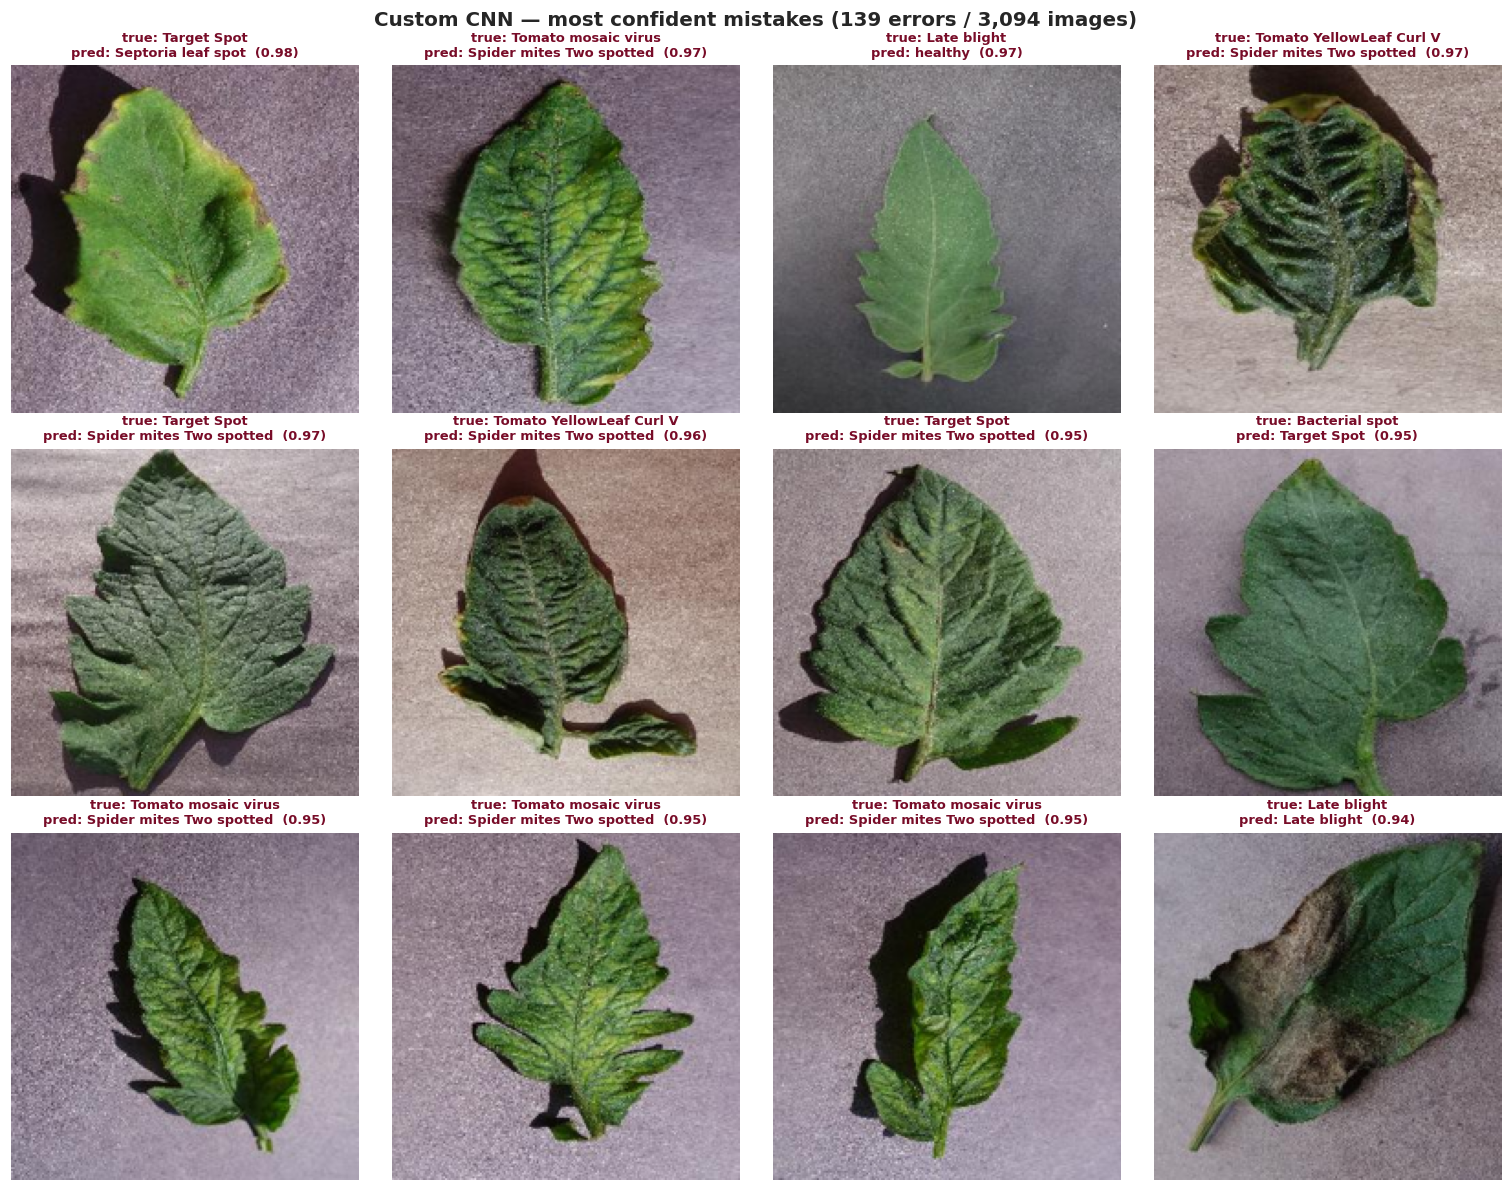
\includegraphics[width=0.9\textwidth]{15_error_gallery.png}
\caption{The twelve most confidently wrong predictions on the test set (Custom CNN).}
\label{fig:errorgallery}
\end{figure}

\section{Explainability -- Grad-CAM}
Grad-CAM~\cite{selvaraju2017gradcam} was used to generate class-discriminative
activation maps for the model's predictions, highlighting the image regions
that most influenced a given classification decision.

\begin{figure}[H]
\centering
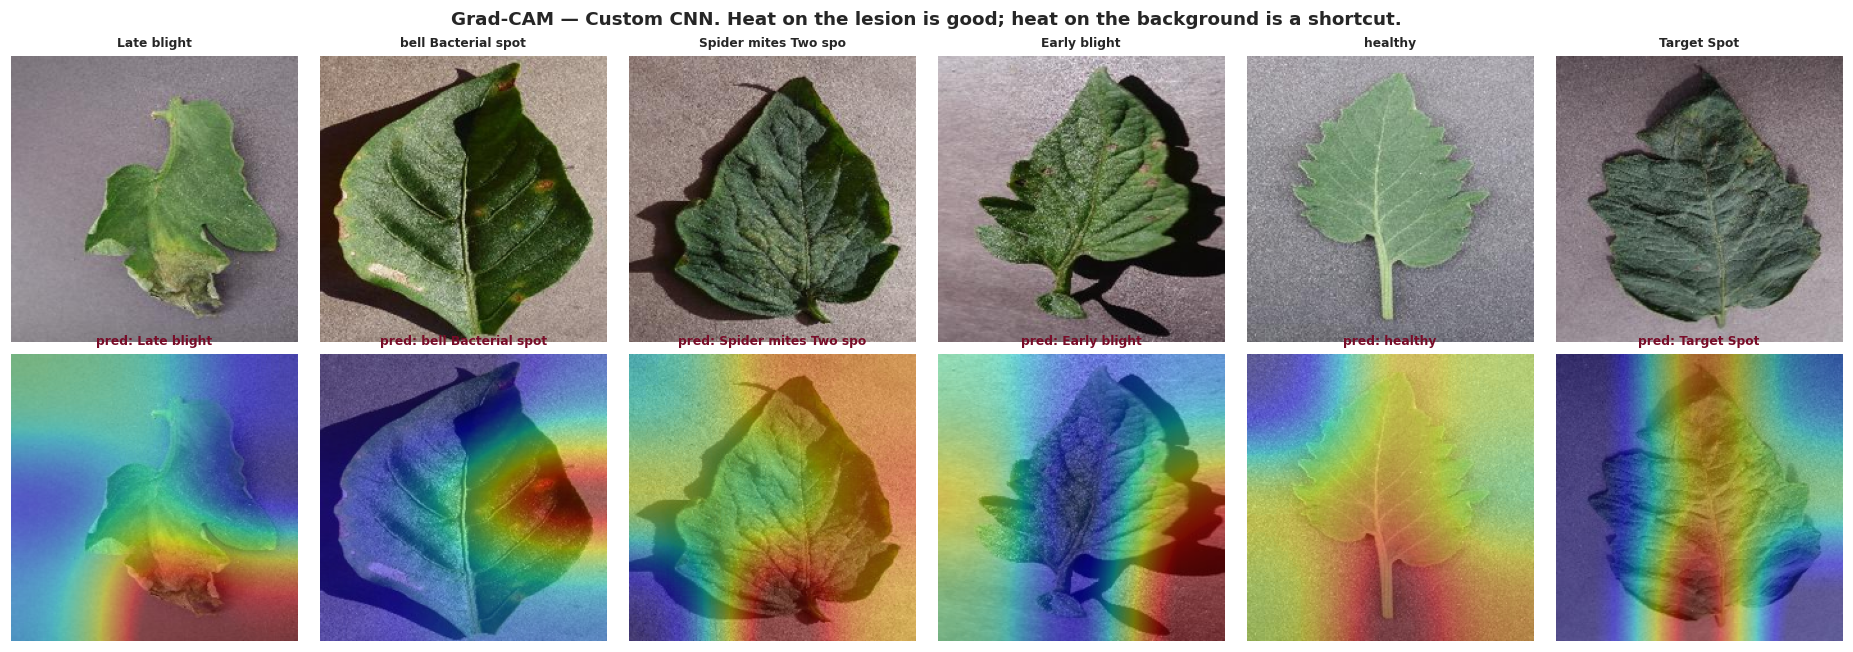
\includegraphics[width=0.9\textwidth]{16_gradcam.png}
\caption{Grad-CAM class-activation visualizations for a sample of predictions.}
\label{fig:gradcam}
\end{figure}

\section{Example Inference}
\begin{figure}[H]
\centering
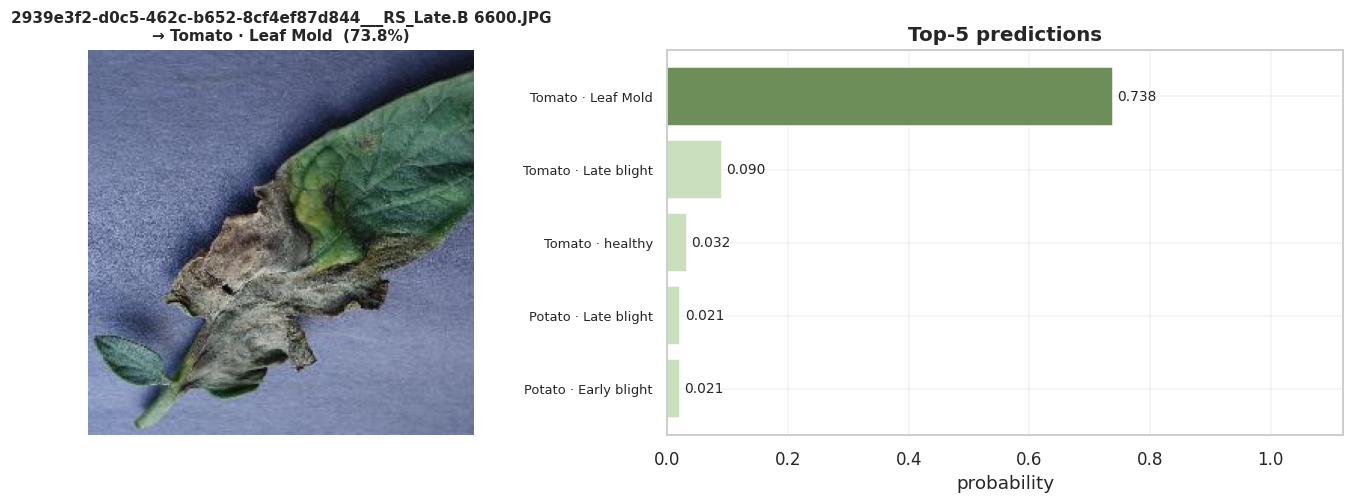
\includegraphics[width=0.85\textwidth]{demo_pred_1.png}
\caption{Example single-image inference with top-5 predicted probabilities.}
\label{fig:demopred}
\end{figure}

\section{On-Device Deployment: TFLite Fidelity and Latency}
\begin{table}[H]
\centering
\caption{Exported model sizes.}
\begin{tabular}{@{}lrrrrr@{}}
\toprule
\textbf{Model} & \textbf{.keras (MB)} & \textbf{.h5 (MB)} & \textbf{TFLite fp32 (MB)} & \textbf{TFLite fp16 (MB)} & \textbf{Params (M)} \\
\midrule
Custom CNN & 130.97 & 130.99 & 43.62 & 21.82 & 10.90 \\
EfficientNetB3 & 91.05 & 90.45 & 44.34 & 22.27 & 11.18 \\
\bottomrule
\end{tabular}
\end{table}

\begin{table}[H]
\centering
\caption{TFLite export fidelity and CPU latency (250-image subset).}
\begin{tabular}{@{}llrrrr@{}}
\toprule
\textbf{Model} & \textbf{Variant} & \textbf{TFLite acc.} & \textbf{$\Delta$ vs.\ Keras} & \textbf{Agreement} & \textbf{ms / image (CPU)} \\
\midrule
Custom CNN & fp32 & 94.40\% & $-2.40$pp & 96.8\% & 177.6 \\
Custom CNN & fp16 & 94.40\% & $-2.40$pp & 96.8\% & 176.1 \\
EfficientNetB3 & fp32 & 90.00\% & $-0.80$pp & 96.4\% & 41.0 \\
EfficientNetB3 & fp16 & 90.00\% & $-0.80$pp & 96.4\% & 41.6 \\
\bottomrule
\end{tabular}
\label{tab:tflite}
\end{table}

Two things are worth noting. First, fp16 quantization roughly halves file
size (Custom CNN: 43.62~MB $\to$ 21.82~MB) with \emph{no} measurable further
accuracy loss beyond fp32 -- the sensible default for a bandwidth- or
storage-constrained deployment. Second, despite having a comparable parameter
count, EfficientNetB3 is over \textbf{4$\times$ faster} on CPU
(41.0~ms/image vs.\ 177.6~ms/image) -- its architecture uses far cheaper
depthwise-separable convolutions than the Custom CNN's large dense
$3\times3$ convolutions at full $224\times224$ resolution in its early
layers. This is a genuine accuracy/latency trade-off a deployment could
reasonably make differently for, e.g., a low-power mobile device.

\section{Output Screens}
The following screens show the deployed Streamlit application. \emph{(Placeholders --
capture these by running \texttt{streamlit run App.py} and replacing each box
with the corresponding screenshot before submission.)}

\ScreenshotPlaceholder{Home tab -- landing page and workflow overview.}{4.5}
\ScreenshotPlaceholder{About tab -- crop/condition reference table.}{4.5}
\ScreenshotPlaceholder{Disease Recognition tab -- image upload and prediction result with confidence and severity.}{5}
\ScreenshotPlaceholder{Location mode selection (manual / GPS) and weather-context panel.}{5}
\ScreenshotPlaceholder{Generated localized treatment plan.}{4.5}
\ScreenshotPlaceholder{Audio playback of the spoken diagnosis / treatment summary.}{3.5}

% ============================================================================
\chapter{Limitations and Future Enhancements}
% ============================================================================

\section{Limitations}
\begin{itemize}[leftmargin=*]
    \item \textbf{Lab-to-field generalization gap.} PlantVillage is an easy
    benchmark by design -- uniform lighting, a single centred leaf, and a
    near-constant background (Section~4.2, Fig.~\ref{fig:meanimage}).
    Accuracy above 95\% on its held-out split, as achieved here, is expected,
    and is \emph{not} evidence that the model works equally well on a real
    farmer's photograph. Published work consistently finds that models
    trained purely on PlantVillage lose substantial accuracy -- often falling
    to 30--50\% -- on field-collected image sets such as
    PlantDoc~\cite{singh2020plantdoc}. This is the single most important
    caveat on the results in Chapter~6.
    \item \textbf{Class coverage.} The evaluated model covers 15
    classes across three crops (Pepper, Potato, Tomato); it does not cover
    other crops or diseases outside this subset.
    \item \textbf{Single-leaf, single-disease assumption.} The pipeline
    assumes one leaf, one dominant condition, per uploaded image; it does not
    detect multiple co-occurring diseases or aggregate a whole-plant/whole-field
    assessment from several photos.
    \item \textbf{External-API dependency.} The treatment-plan, weather, and
    geocoding features require network connectivity and depend on the
    continued availability and free-tier limits of third-party APIs (Groq,
    Open-Meteo, Nominatim), which the classification step itself does not.
    \item \textbf{No confidence-based abstention (yet).} Although the model
    is well-calibrated overall (ECE 0.0314, Section~6.6) and shows a clear
    confidence gap between correct and incorrect predictions (0.936 vs.\
    0.664), the current application surfaces every prediction rather than
    routing low-confidence cases to a human agronomist or a ``try another
    photo'' prompt.
\end{itemize}

\section{Future Enhancements}
\begin{itemize}[leftmargin=*]
    \item \textbf{Field-image validation and fine-tuning.} Evaluate against
    (and fine-tune on) a field-collected dataset such as PlantDoc, and report
    that number -- not the PlantVillage number -- as the deployment-readiness
    metric.
    \item \textbf{Confidence-based abstention.} Use the risk--coverage
    relationship implied by Fig.~\ref{fig:calibration} to route low-confidence
    predictions to a ``diagnosis unclear'' state instead of a possibly wrong
    label.
    \item \textbf{Broader class and crop coverage,} extending beyond the
    current 15-class Pepper/Potato/Tomato subset.
    \item \textbf{Offline / low-connectivity mode,} caching recent weather
    and a generic (non-personalized) treatment library for use when the LLM,
    weather, or geocoding APIs are unreachable.
    \item \textbf{Native mobile application} built directly on the exported
    fp16 TFLite model, avoiding a network round-trip for the classification
    step entirely.
    \item \textbf{Active learning / continuous improvement,} collecting
    (consented) field photos submitted through the app to progressively
    close the lab-to-field gap described above.
\end{itemize}

% ============================================================================
\chapter{Conclusion}
% ============================================================================

This project set out to build not just a disease classifier, but a complete,
usable decision-support pipeline for farmers: diagnosis, severity, and a
localized, weather-aware treatment plan, delivered bilingually with audio
support. On the modeling side, two architectures were trained and rigorously
compared under an identical, leakage-checked protocol; the simpler,
from-scratch CNN outperformed EfficientNetB3 transfer learning on this
dataset (95.51\% vs.\ 87.10\% test accuracy, 94.59\% vs.\ 86.92\% macro-F1),
was well-calibrated (ECE 0.0314), and exported to a quantized on-device format
with verified, near-lossless fidelity. On the application side, the
classifier was embedded in a system that reasons about severity from disease
facts rather than model confidence, and produces treatment advice grounded in
the farmer's actual location and current weather -- output that is
substantially more actionable than a bare class label.

The report has also tried to be honest about what these results do and do not
show: the headline accuracy is a PlantVillage number, and the literature is
clear that such numbers do not transfer directly to field conditions. That
gap, and the concrete steps to close it (Chapter~7), are the natural next
phase of this work.

% ============================================================================
%  APPENDICES
% ============================================================================
\appendix
\renewcommand{\thechapter}{\Alph{chapter}}
\titleformat{\chapter}[hang]{\normalfont\Huge\bfseries}{Appendix \thechapter.}{18pt}{\Huge}

\chapter{Dataset Class List and Per-Split Image Counts}
\begin{table}[H]
\centering
\caption{Per-class image counts by split.}
\begin{tabular}{@{}lrrr@{}}
\toprule
\textbf{Class} & \textbf{Train} & \textbf{Val} & \textbf{Test} \\
\midrule
Pepper -- Bacterial spot & 698 & 149 & 150 \\
Pepper -- healthy & 1{,}035 & 222 & 221 \\
Potato -- Early blight & 700 & 150 & 150 \\
Potato -- Late blight & 700 & 150 & 150 \\
Potato -- healthy & 106 & 23 & 23 \\
Tomato -- Bacterial spot & 1{,}489 & 319 & 319 \\
Tomato -- Early blight & 700 & 150 & 150 \\
Tomato -- Late blight & 1{,}331 & 285 & 285 \\
Tomato -- Leaf Mold & 666 & 143 & 143 \\
Tomato -- Septoria leaf spot & 1{,}240 & 266 & 265 \\
Tomato -- Spider mites & 1{,}173 & 251 & 252 \\
Tomato -- Target Spot & 983 & 210 & 211 \\
Tomato -- Yellow Leaf Curl Virus & 2{,}245 & 482 & 481 \\
Tomato -- mosaic virus & 261 & 56 & 56 \\
Tomato -- healthy & 1{,}109 & 238 & 238 \\
\midrule
\textbf{Total} & \textbf{14{,}436} & \textbf{3{,}094} & \textbf{3{,}094} \\
\bottomrule
\end{tabular}
\end{table}

\begin{table}[H]
\centering
\caption{Balanced class weights applied during training.}
\begin{tabular}{@{}lrr@{}}
\toprule
\textbf{Class} & \textbf{Train images} & \textbf{Weight} \\
\midrule
Potato -- healthy & 106 & 9.079 \\
Tomato -- mosaic virus & 261 & 3.687 \\
Tomato -- Leaf Mold & 666 & 1.445 \\
Pepper -- Bacterial spot & 698 & 1.379 \\
Potato -- Late blight & 700 & 1.375 \\
Tomato -- Early blight & 700 & 1.375 \\
Potato -- Early blight & 700 & 1.375 \\
Tomato -- Target Spot & 983 & 0.979 \\
Pepper -- healthy & 1{,}035 & 0.930 \\
Tomato -- healthy & 1{,}109 & 0.868 \\
Tomato -- Spider mites & 1{,}173 & 0.820 \\
Tomato -- Septoria leaf spot & 1{,}240 & 0.776 \\
Tomato -- Late blight & 1{,}331 & 0.723 \\
Tomato -- Bacterial spot & 1{,}489 & 0.646 \\
Tomato -- Yellow Leaf Curl Virus & 2{,}245 & 0.429 \\
\bottomrule
\end{tabular}
\end{table}

\chapter{Data Pipeline and Augmentation -- Code Listing}
\lstinputlisting[language=Python, caption={Input pipeline and augmentation stack (excerpted from the training notebook).}]{listings/input_pipeline.py}

\chapter{Full Training Configuration -- Code Listing}
\lstinputlisting[language=Python, caption={Complete \texttt{CFG} configuration block (training notebook).}]{listings/cfg_block.py}

% ============================================================================
%  REFERENCES  (numbered in order of first appearance, per report convention)
% ============================================================================
\begin{thebibliography}{99}

\bibitem{mohanty2016}
S.~P. Mohanty, D.~P. Hughes, and M.~Salath\'e,
``Using Deep Learning for Image-Based Plant Disease Detection,''
\emph{Frontiers in Plant Science}, vol.~7, article 1419, 2016.

\bibitem{ferentinos2018}
K.~P. Ferentinos,
``Deep learning models for plant disease detection and diagnosis,''
\emph{Computers and Electronics in Agriculture}, vol.~145, pp.~311--318, 2018.

\bibitem{plantvillage-kaggle}
Kaggle dataset: \emph{PlantVillage Dataset} (mirrored by user \texttt{emmarex}),
\url{https://www.kaggle.com/datasets/emmarex/plantdisease}, accessed 2026.

\bibitem{tan2019efficientnet}
M.~Tan and Q.~V. Le,
``EfficientNet: Rethinking Model Scaling for Convolutional Neural Networks,''
in \emph{Proceedings of the 36th International Conference on Machine Learning
(ICML)}, 2019.

\bibitem{selvaraju2017gradcam}
R.~R. Selvaraju, M.~Cogswell, A.~Das, R.~Vedantam, D.~Parikh, and D.~Batra,
``Grad-CAM: Visual Explanations from Deep Networks via Gradient-based
Localization,'' in \emph{Proceedings of the IEEE International Conference on
Computer Vision (ICCV)}, 2017.

\bibitem{singh2020plantdoc}
D.~Singh, N.~Jain, P.~Jain, P.~Kayal, S.~Kumawat, and N.~Batra,
``PlantDoc: A Dataset for Visual Plant Disease Detection,''
in \emph{Proceedings of the 7th ACM IKDD CoDS and 25th COMAD}, 2020,
pp.~249--253.

\bibitem{streamlit}
Streamlit Inc., \emph{Streamlit Documentation},
\url{https://docs.streamlit.io/}, accessed 2026.

\bibitem{tensorflow}
M.~Abadi et al., \emph{TensorFlow: Large-Scale Machine Learning on
Heterogeneous Systems}, 2015, \url{https://www.tensorflow.org/}.

\bibitem{openmeteo}
Open-Meteo, \emph{Open-Meteo Weather Forecast API Documentation},
\url{https://open-meteo.com/en/docs}, accessed 2026.

\bibitem{nominatim}
OpenStreetMap Foundation, \emph{Nominatim Geocoding API Documentation},
\url{https://nominatim.org/release-docs/latest/}, accessed 2026.

\bibitem{groq}
Groq Inc., \emph{Groq API Documentation},
\url{https://console.groq.com/docs}, accessed 2026.

\bibitem{gtts}
P.~N. Didier, \emph{gTTS: Python library and CLI tool for Google Text-to-Speech},
\url{https://gtts.readthedocs.io/}, accessed 2026.

\end{thebibliography}

\end{document}
